% ----------------------------------------------------
% DAB Processing
% ----------------------------------------------------
\documentclass[class=report,11pt,crop=false]{standalone}
% Page geometry
\usepackage[a4paper,margin=25mm,top=25mm,bottom=25mm]{geometry}

% Font choice
\usepackage{lmodern}

% Use IEEE bibliography style
\bibliographystyle{IEEEtran}

% Line spacing
\usepackage{setspace}
\setstretch{1.20}

% Ensure UTF8 encoding
\usepackage[utf8]{inputenc}

% Language standard (not too important)
\usepackage[english]{babel}

% Skip a line in between paragraphs
\usepackage{parskip}

% For the creation of dummy text
\usepackage{blindtext}

% Math
\usepackage{amsmath}

% Header & Footer stuff
\usepackage{fancyhdr}
\pagestyle{fancy}
\fancyhead{}
\fancyhead[R]{\nouppercase{\rightmark}}
\fancyfoot{}
\fancyfoot[C]{\thepage}
\renewcommand{\headrulewidth}{0.0pt}
\renewcommand{\footrulewidth}{0.0pt}
\setlength{\headheight}{13.6pt}

% Page geometry
\usepackage[a4paper,top=25mm,bottom=25mm]{geometry}

% Epigraphs
\usepackage{epigraph}
\setlength\epigraphrule{0pt}

% Hyperlinks & References
\usepackage{hyperref}
\hypersetup{
    colorlinks=true,
    linkcolor=blue,
    filecolor=blue,      
    urlcolor=blue,
    citecolor=blue,
}
\urlstyle{same}

% Automatically correct front-side quotes
\usepackage[autostyle=false, style=american]{csquotes}
\MakeOuterQuote{"}

% Graphics
\usepackage{graphicx}
\graphicspath{{Images/}{../Images/}}

% Colour
\usepackage{color}
\usepackage[usenames,dvipsnames]{xcolor}

% SI units
\usepackage{siunitx}

% Microtype goodness
\usepackage{microtype}

% Listings
\usepackage{listings}
\definecolor{backgroundColour}{RGB}{250,250,250}
\definecolor{commentColour}{RGB}{73, 175, 102}
\definecolor{identifierColour}{RGB}{196, 19, 66}
\definecolor{stringColour}{RGB}{252, 156, 30}
\definecolor{keywordColour}{RGB}{50, 38, 224}
\definecolor{lineNumbersColour}{RGB}{127,127,127}
\lstset{ 
  language=Matlab,
  captionpos=b,
  backgroundcolor=\color{backgroundColour},
  basicstyle=\footnotesize,        % the size of the fonts that are used for the code
  breakatwhitespace=false,         % sets if automatic breaks should only happen at whitespace
  breaklines=true,                 % sets automatic line breaking
  postbreak=\mbox{\textcolor{red}{$\hookrightarrow$}\space},
  commentstyle=\color{commentColour},    % comment style
  identifierstyle=\color{identifierColour},
  stringstyle=\color{stringColour},
   keywordstyle=\color{keywordColour},       % keyword style
  %escapeinside={\%*}{*)},          % if you want to add LaTeX within your code
  extendedchars=true,              % lets you use non-ASCII characters; for 8-bits encodings only, does not work with UTF-8
  frame=single,	                   % adds a frame around the code
  keepspaces=true,                 % keeps spaces in text, useful for keeping indentation of code (possibly needs columns=flexible)
  morekeywords={*,...},            % if you want to add more keywords to the set
  numbers=left,                    % where to put the line-numbers; possible values are (none, left, right)
  numbersep=5pt,                   % how far the line-numbers are from the code
  numberstyle=\tiny\color{lineNumbersColour}, % the style that is used for the line-numbers
  rulecolor=\color{black},         % if not set, the frame-color may be changed on line-breaks within not-black text (e.g. comments (green here))
  showspaces=false,                % show spaces everywhere adding particular underscores; it overrides 'showstringspaces'
  showstringspaces=false,          % underline spaces within strings only
  showtabs=false,                  % show tabs within strings adding particular underscores
  stepnumber=1,                    % the step between two line-numbers. If it's 1, each line will be numbered
  tabsize=2,	                   % sets default tabsize to 2 spaces
  %title=\lstname                   % show the filename of files included with \lstinputlisting; also try caption instead of title
}

% Caption stuff
\usepackage{caption}
\usepackage{subcaption}

\makenoidxglossaries

\newacronym{radar}{RADAR}{Radio Detection and Ranging}
\newacronym{dab}{DAB}{Digital Audio Broadcasting}
\newacronym{fm}{FM}{Frequency Modulation}
\newacronym{am}{AM}{Amplitude Modulation}
\newacronym{fdm}{FDM}{Frequency Division Multiplexing}
\newacronym{ofdm}{OFDM}{Orthogonal Frequency Division Multiplexing}
\newacronym{cofdm}{COFDM}{Coded Orthogonal Frequency Division Multiplexing}
\newacronym{dvbt2}{DVB–T2}{Digital Video Broadcasting — Second Generation Terrestrial}
\newacronym{em}{EM}{electromagnetic}
\newacronym{icasa}{ICASA}{Independent Communications Authority of South Africa}
\newacronym{ioo}{IOO}{Illuminators of Opportunity}
\newacronym{pr}{PR}{Passive Radar}
\newacronym{qpsk}{QPSK}{Differential Quadrature Phase-Shift Keying}
\newacronym{dqpsk}{DQPSK}{Differential Quadrature Phase-Shift Keying}
\newacronym{etsi}{ETSI}{European Telecommunications Standards Institute}
\newacronym{psk}{PSK}{Phase Shift Keying}
\newacronym{ask}{ASK}{Amplitude-Shift Keying}
\newacronym{fsk}{FSK}{Frequency-Shift Keying}
\newacronym{iq}{IQ}{In-phase and Quadrature}
\newacronym{prs}{PRS}{Phase Reference Symbol}
\newacronym{dft}{DFT}{Discrete Fourier Transform}
\newacronym{fft}{FFT}{Fast Fourier Transform}
\begin{document}
\ifstandalone
\tableofcontents
\fi
% ----------------------------------------------------
\chapter{Digital Audio Broadcasting: Processing Chain Design}
\epigraph{Nobody can build you the bridge over which you must cross the river of life, nobody but you alone.}%
    {\emph{---Friedrich Nietzsche}}
% ----------------------------------------------------

This chapter details the core design component of the project: a \gls{dab} processing chain. While the broader context of this report falls within the realm of \gls{pr}, the fundamental task at hand was to demodulate and remodulate a given \gls{dab} signal, in order to create a perfect reference signal of given recorded data. Fortunately, as outlined in the previous chapter, not all of the intricacies of the \gls{dab} standard were required to be understood or even considered for integration into a passive radar chain.

The design of the chain involved studying the \gls{dab} standard document from the \gls{etsi}~\cite{dabstandard}, as well as using a reference signal which was known to be perfectly modulated for initial testing. For some functionality, real-world data was also used for design and testing. For the sake of simplicity, the entire chain---including all the dimensions shown in this chapter---was designed around \gls{dab} Mode 1. Nonetheless, altering the chain for implementation with other modes will be trivial. All MATLAB functions were designed with a \texttt{dab\_mode} input, if necessary, to allow for easy changes in future designs. Note, however, that this mode input parameter is not shown in any of the upcoming diagrams.

\section{Overview}
Within the \gls{dab} processing chain, three main functional blocks were identified: pre-processing, demodulation, and remodulation. The first block reads in a \gls{dab} recording of \gls{iq} data saved as a binary file, and outputs a single \gls{dab} frame from this file. This frame can then be input to the demodulate block, which extracts the \gls{dab} data from it. This data is not the decoded information from the \gls{dab} recording---such as the audio signal---rather, it is simply an extracted bitstream. This bitstream can then be perfectly reconstructed as a \gls{dab} frame, by the remodulate block. A diagrammatic overview of this chain is given in Figure~\ref{fig:BD_Overview_All}.

\begin{figure}[htbp]
  \centering
  \captionsetup{type=figure}
  \def\svgwidth{\linewidth}
  {\setstretch{0.7} % Line spacing
      \input{../Images/BD_Overview_All-embed.pdf_tex}}
  \caption{Block diagram showing entire DAB processing chain}
  \label{fig:BD_Overview_All}
\end{figure}

Notice in the figure that each of the aforementioned blocks---the pre-process, demodulate, and remodulate blocks---was created from a collection of smaller sub-blocks. These sub-blocks were designed to perform simpler tasks individually, and were written as relatively short MATLAB functions. This atomic-function approach had a host of benefits for the design, debugging, and validation of the chain, and added layers of abstraction for the larger system.

Each of the three blocks will be unpacked in the sections that follow this one, with subsections dedicated to the relevant sub-blocks.

% ##############################################################################################################################
%   P R E - P R O C E S S I N G
% ##############################################################################################################################
\section{Pre-processing \label{sect:dab-proc_preprocessing}}
\subsection{Overview}
The pre-processing chain was designed to read in an \gls{iq} data file, synchronize it appropriately, and extract a single frame from it. Note that in an actual \gls{pr} system---where this \gls{dab} processing chain would be only a small part of a larger chain---this block would be markedly different. If nothing else, a real-world chain would probably stream the \gls{iq} data, rather than read it from a pre-recorded file. Moreover, a real chain might process several \gls{dab} frames at once. However, such details are largely context-specific, and it would be superfluous to include every use-case in this report. Importantly, the other two blocks---used to demodulate and remodulate---would mostly remain the same in various other scenarios. Thus, to make matters simpler, the pre-processing block was designed to be straightforward: to read in data and extract a single frame. That is not to say the block is trivial, and there were some important design decisions made for it.

The pre-processing block has four key stages: reading in \gls{iq} data from a binary file, resampling this data if necessary, detecting the location of the \gls{prs} and thus synchronizing the recording, and then extracting a \gls{dab} frame accordingly. This pipeline is shown graphically in Figure~\ref{fig:BD_Preprocess_All}.

\begin{figure}[htbp]
    \centering
    \captionsetup{type=figure}
    \def\svgwidth{\linewidth}
    {\setstretch{0.7} % Line spacing
        \input{../Images/BD_Preprocess_All-embed.pdf_tex}}
    \caption{Block diagram showing preprocessing section of processing chain}
    \label{fig:BD_Preprocess_All}
\end{figure}

\subsection{Reading IQ data from file \label{subsect:dab-proc_iq-read}}
The first sub-block is called \texttt{iq\_read}, and, as mentioned previously, would likely be very different in a real \gls{pr} chain. Nonetheless, here it reads in a \gls{dab} recording from a binary file, and outputs so-called "raw" \gls{iq} data. No changes are made to this data in this function, and it essentially just abstracts MATLAB's file-handling functionality conveniently.

As a minor note, one must remember that a \gls{dab} recording contains \gls{iq} data, which is complex-valued. Since a binary file cannot store such a datatype, it will usually be stored as pairs of numbers. To read this correctly in MATLAB, one can use the simple code shown in Listing~\ref{code:iq_read}.

\begin{lstlisting}[caption={Creating a complex data array with the values read from a binary file},label={code:iq_read}]
iq_data_raw = data_from_file(1:2:end) + 1j*data_from_file(2:2:end);
\end{lstlisting}

Though it is not shown in the pre-processing block diagrams, the MATLAB function for \texttt{iq\_read} also included some other input parameters for convenience, including the data-type of the binary file, the offset to skip in the file's data, the number of frames to read, and so on.

A perfect \gls{dab} recording that would be output from the \texttt{iq\_read} function is shown in Figure~\ref{fig:plots/perfect-dab-signal}, showing a handful of \gls{dab} frames. Notice the separation of successive frames by the distinct null symbols.

\begin{figure}[htbp]
  \centering
  \captionsetup{type=figure}
  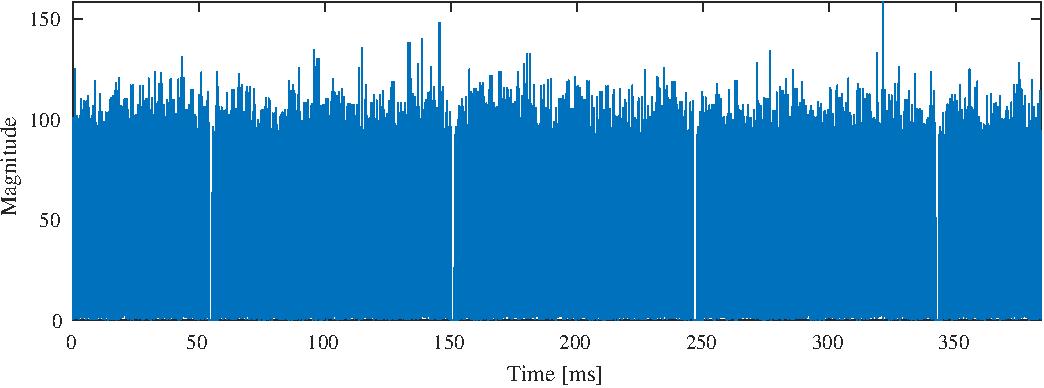
\includegraphics[width=\linewidth]{plots/perfect-dab-signal.pdf}
  \caption{Time-domain plot of a handful of frames of a perfect \gls{dab} signal}
  \label{fig:plots/perfect-dab-signal}
\end{figure}

\subsection{Resampling IQ data \label{subsect:dab-proc_iq-resample}}
In order for one to utilise the \gls{fft} to demodulate an \gls{ofdm} symbol, certain requirements must be met. Recall that the window for a single symbol, notated as \(T_u\), is 2048 samples for \gls{dab} Mode 1. This means that a 2048-point \gls{fft} must be used, with a resulting 2048 points in the frequency domain. Recall also that \gls{ofdm} has a strict requirement for the spacing between adjacent carriers---\(1 \si{\kilo \hertz}\) for \gls{dab} Mode1. Notice, then, if the sample rate for the original signal is precisely set at \(F_s = 2.048 \si{\mega \hertz}\), for \gls{dab} Mode 1, then the bins from the \gls{fft} will be perfectly aligned on the \gls{ofdm} carriers---enabling proper demouldation.

However, in a real-world scenario, the desired sampling rate might not necessarily be used in the receiver. Thus, in such a situation, the \gls{iq} data must be resampled. Consider an original sampling rate of \(F_s\), a desired sampling rate of \(\tilde{F_s} = 2.048 \si{\mega \hertz}\), with \(F_s \ne \tilde{F_s}\), and with
\begin{equation}
  \frac{\tilde{F_s}}{F_s} = \frac{P}{Q}
\end{equation}
where \(P\) and \(Q\) are integers---preferably chosen such that \(P/Q\) is in its most reduced fractional form. Resampling, then, is equivalent to upsampling by a factor of \(P\), and thereafter downsampling by a factor of \(Q\).

Fortunately, MATLAB provides a neat abstraction of this process with the \texttt{resample(X, P, Q)} function, where \(X\) is a uniformly sampled signal, and \(P\) and \(Q\) are as defined above.

% -----------------
\subsection{Frame Synchronization via Phase Reference Symbol Detection \label{subsect:dab-proc_prs-detect}}

One of the most important parts of the entire \gls{dab} processing chain is correct time-synchronization. If the frame from the pre-processing block is misaligned, the entire demodulation process can break due to misalignment of the \gls{ofdm} symbols, thus causing havoc in the \gls{dqpsk} demodulation. Fortunately, the inclusion of a guard interval with cyclic prefixing provides some leeway, but errors can easily arise if one is not careful. It will later be shown how negatively a result is affected by the incorrect alignment of a \gls{dab} frame.

There are two mechanisms built into the \gls{dab} signal for synchronization, namely the \acrfull{ns} and the \acrfull{prs}. As specified in the \gls{dab} standard document~\cite{dabstandard}, the former symbol is to be used for so-called "coarse" synchronization---detecting an approximate location of the frame's beginning; whereas the latter symbol is used for "fine" synchronization---detecting the exact sample at which the frame starts. 

Naturally, for each of these detection processes, one cannot consider the entirety of a signal---stretching back from the dawn of time to the eventual collapse of the universe far in the future---more than just practically impossible, it would be unnecessary. Instead only a chunk of the data can be considered at once, as a subset of the longer signal. This process is termed "windowing," where the signal is truncated to a finite domain over which it will be examined. Let the length of this window be notated\footnote{The is not necessarily standardised notation.} as \(T_w\), and let the interval between successive windows be called the "advancement interval", \(T_a\). Graphically, these values are depicted in Figure~\ref{fig:window_advance_illustration}.

\begin{figure}[htbp]
  \centering
  \captionsetup{type=figure}
  \def\svgwidth{\linewidth}
  {\setstretch{0.7} % Line spacing
      \input{../Images/window_advance_illustration.pdf_tex}}
      \caption{}
      \label{fig:window_advance_illustration}
\end{figure}

In order not to skip any sections of the signal, it is clear that the following must hold:
\begin{equation}
  T_a \le T_w
\end{equation}

Consider firstly the detection of the \gls{ns}. Recall that this symbol is a period in the signal during which all \gls{ofdm} carriers are turned off and no power is transmitted. On the receiver's end, there will still be noise recorded from the environment and elsewhere, but the received power over the length of the null symbol, \(T_\textrm{null}\), will be significantly less than in other parts of the signal. Hence, in order to detect this symbol, one can calculate the average power starting at index \(n_0\) over a window of~\(T_w = T_\textrm{null}\). Let this be notated as \(P_{n_0}\), and calculated as:
\begin{equation}
  P_{n_0} = \frac{1}{T_w} \cdot \sum^{n_0 + T_w - 1}_{n=n_0} \left| x[n] \right|^2
\end{equation}
where \(x[n]\) is the sampled signal, windowed on the domain \([n_0, n_0 + T_w)\). This window can be moved along the original signal, in increments of \(T_a\). Since the \gls{ns} only provides a coarse result, and further synchronisation steps would always be required, the specific value of \(T_a\) is not too important, provided it is less than or equal to \(T_w\). When the average power of a window decreases below a particular threshold---for example, it could be compared to the average power of a \emph{frame}-lengthed chunk of the signal---the \gls{ns} has been approximately detected. If things are working correctly, the symbol detection should occur within the first \(T_f\) samples---if not, there is a problem.

An outline of the coarse detection process is given in Algorithm~\ref{alg:null_symbol_detect}.

\begin{figure}[ht]
  \vspace{0.5cm}
  \centering
  \captionsetup{type=figure}
  \begin{minipage}{.75\linewidth}
    \begin{algorithm}[H]
      \caption{Coarse Frame Synchronization via Null Symbol Detection\label{alg:null_symbol_detect}}

      \DontPrintSemicolon
      \SetAlgoLined
      \SetKwInOut{Input}{input}\SetKwInOut{Output}{output}\SetKwInOut{Parameter}{parameter}

      \Input{A sampled \gls{dab} signal, $x[n]$}
      \Output{The approximate index of the first \acrlong{ns}}
      \Parameter{Threshold constant, $\gamma > 1$}

      \BlankLine
          \Begin{
          $P_\textrm{frame} \leftarrow \frac{1}{T_f} \cdot \sum^{T_f - 1}_{n=0} \left| x[n] \right|^2$\;
          $n_0 \leftarrow 0$ \;
          \While(){$(n_0 < T_f)$}{
            $P_{n_0} \leftarrow \frac{1}{T_w} \cdot \sum^{n_0 + T_w - 1}_{n=n_0} \left| x[n] \right|^2$ \;

            \eIf{$(P_\mathrm{frame} > \gamma P_{n_0})$}{
              \Return $n_0$ \;
            }{
              $n_0 \leftarrow n_0 + T_a$ \;
            } 
          }
        }
      \vspace{0.5cm}
    \end{algorithm}
  \end{minipage}
\end{figure}

Consider next the detection of the \gls{prs}. Because this symbol is precisely defined by the \gls{dab} standard, it was known \emph{a priori} and thus could be detected via a Matched Filtering process, which is essentially a time-domain correlation. Conceptually, this entailed designing a filter, \(H(\omega)\), based on the \gls{prs}:
\begin{equation}
  H(\omega) = R^*(\omega)
\end{equation}
where \(R^*(\omega)\) was the conjugate of the continuous-time Fourier transform of the \gls{prs}. Of course, since the system was implemented digitally, the filter had to be defined discretely:
\begin{equation}
  H[k] = R^*[k] = \mathrm{DFT} \{ r[n] \}^*
\end{equation}

Since the \gls{dft} is a \(\mathbb{C}^N \rightarrow \mathbb{C}^N\) transformation, the filter length---and thus the window size, \(T_w\)---is constrained to the length of \(r[n]\). This length is equal to \(T_u\), the "useful symbol length" in the \gls{dab} standard.

The output of the Matched Filter in the Fourier domain, \(Y[k]\), for a given input signal, \(x[n]\), can be calculated via a simple Hadamard (pointwise) product:
\begin{equation}
  Y[k] = H[k] \odot X[k] = H[k] \odot \mathrm{DFT} \{ x[n] \}
\end{equation}

The output of this filter in time, \(y[n]\), will contain a peak value at the location within \(x[n]\) where \(r[n]\) is most highly correlated. In an arbitrary section of the \gls{dab} signal, the output will simply be noise, as the signals are not correlated; however, in a section containing the \gls{prs}, the peak value will be noticeably larger than surrounding values, even when using a non-perfect recording. One could detect this peak by comparing it to the average value of the Matched Filter output, for example. Figure~\ref{fig:mf_out_good} shows an example of the filtering process when the \gls{prs} falls within the window of \(x[n]\).

\begin{figure}[htbp]
  \centering
  \captionsetup{type=figure}
  \begin{subfigure}[t]{\textwidth}
    \centering
    \captionsetup{type=figure}
    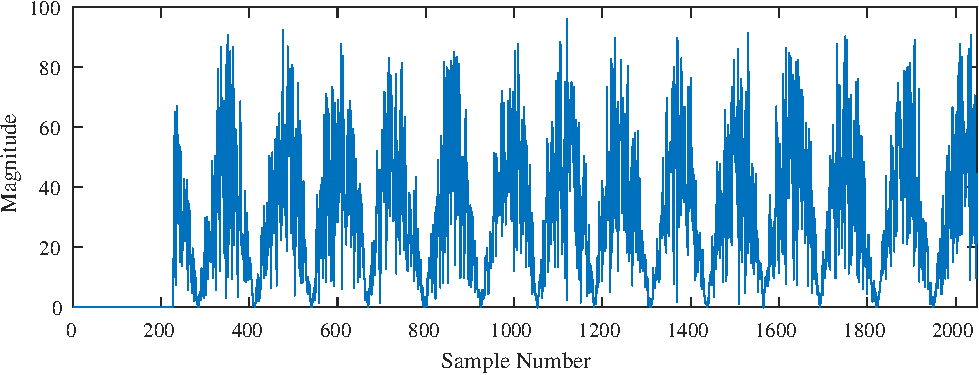
\includegraphics[width=0.7\linewidth]{plots/mf_out_good_signal.pdf}
    \caption{Input to Matched Filter, \(x[n]\)}
    \label{fig:mf_out_good_signal}
  \end{subfigure}%
  \\
  \begin{subfigure}[t]{\textwidth}
    \centering
    \captionsetup{type=figure}
    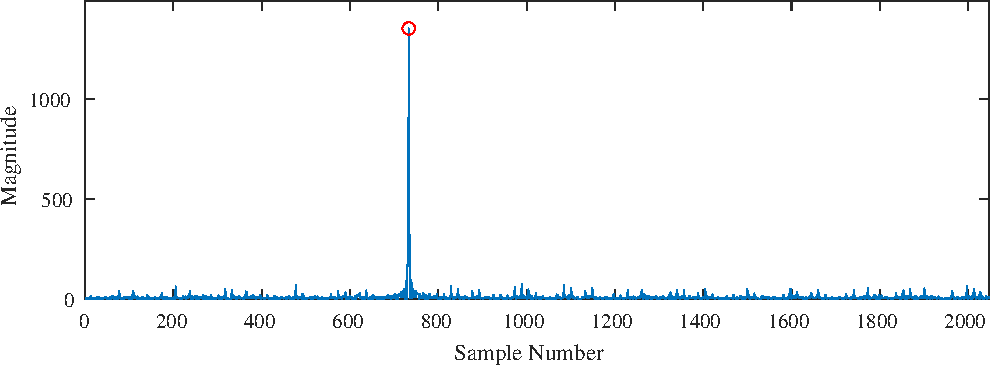
\includegraphics[width=0.7\linewidth]{plots/mf_out_good_peak.pdf}
    \caption{Output from Matched Filter, \(y[n]\), with peak detected}
    \label{fig:mf_out_good_peak}
  \end{subfigure}
  \caption{Plots showing the input to- and output from the Matched Filter, when the \gls{prs} symbol is detected}
  \label{fig:mf_out_good}
\end{figure}

By moving a window of length \(T_w = T_u\) across the input \gls{dab} signal until a peak is detected in the Matched Filter output, one can locate the \gls{prs}---and thus the beginning of the \gls{dab} frame---precisely. This detection should occur within the first \(T_f\) samples. There are two important points to make here. Firstly, note that the magnitude of the Matched Filter's output, \(|y[n]|\), decreases as the offset of the recorded \gls{prs} within the window increases. That is, suppose the \gls{prs} begins at the sample index \(n_p\). If the windowed \gls{dab} signal, \(x[n]\), covers the domain \(n \in [n_p, n_p + T_u]\), then \(x[n]\) is perfectly correlated with the \gls{prs} (ignoring noise in the recording); thus, the output of the Matched Filter will be large. However, as \(n_p\) increases, less of the \gls{prs} signal will be included in \(x[n]\), and the correlation peak will decrease. The smaller the correlation peak, the less distinct it will be from other peaks, and the less likely it will be successfully found.

Secondly, notice that the peak of the Matched Filter output, in Figure~\ref{fig:mf_out_good_peak}, does not occur at the onset of the input signal, \(x[n]\); rather, it occurs around 500 samples later. This was expected, due to the inclusion of a guard interval---since the Matched Filter, \(H[k]\), is defined around the original \gls{prs} signal of length~\(T_u\), without the guard interval. However, unfortunately, this causes an unwanted effect in the detection process. Consider a situation in which \(x[n]\) only contains the guard interval of the \gls{prs}, before the actual "useful" symbol begins, as shown in Figure~\ref{fig:mf_out_prefix-problem_signal}.

\begin{figure}[htbp]
  \centering
  \captionsetup{type=figure}
  \begin{subfigure}[t]{\textwidth}
    \centering
    \captionsetup{type=figure}
    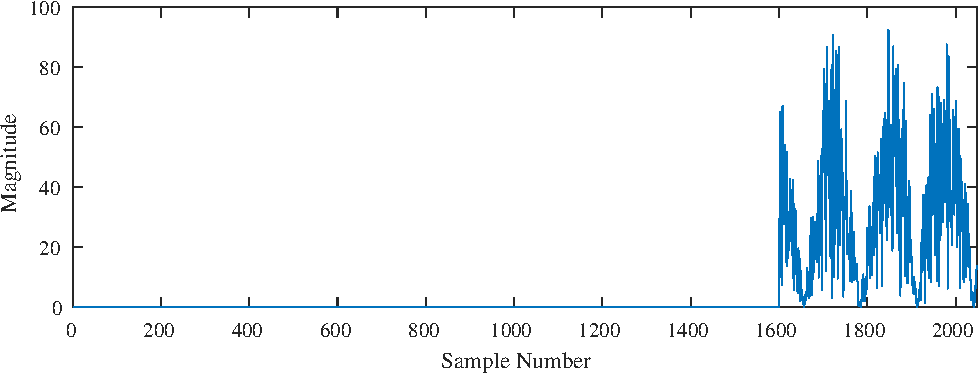
\includegraphics[width=0.7\linewidth]{plots/mf_out_prefix-problem_signal.pdf}
    \caption{Input to Matched Filter, \(x[n]\)}
    \label{fig:mf_out_prefix-problem_signal}
  \end{subfigure}%
  \\
  \begin{subfigure}[t]{\textwidth}
    \centering
    \captionsetup{type=figure}
    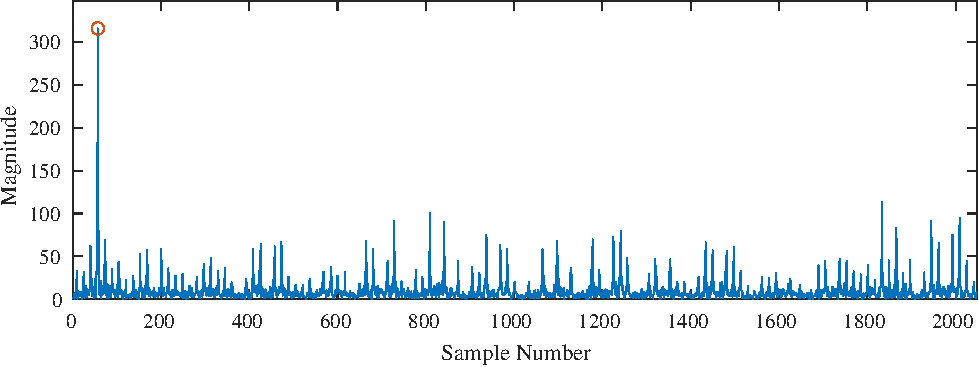
\includegraphics[width=0.7\linewidth]{plots/mf_out_prefix-problem_peak.pdf}
    \caption{Output from Matched Filter, \(y[n]\), with peak erroneously detected}
    \label{fig:mf_out_prefix-problem_peak}
  \end{subfigure}
  \caption{Plots showing the input to- and output from the Matched Filter, when the \gls{prs} symbol is erroneously detected due to the guard interval}
  \label{fig:mf_out_prefix-problem}
\end{figure}

Notice that the peak identified in the Matched Filter output, seen in Figure~\ref{fig:mf_out_prefix-problem_peak}, is erroneous---the actual \gls{prs} has, in fact, not yet begun. Recall that the guard interval is duplicated from the tail-end of the original symbol; thus, the end of the \gls{prs} in the Matched Filter has correlated with the guard interval of the input signal, \(x[n]\). Though this peak is not massive, it can nevertheless be incorrectly identified as the beginning of the \gls{dab} frame.

Both of these points---the decreasing correlation peak, and the guard interval problem---motivate the choice of the advancement interval to be less than the window period. Of course, there is a trade-off, as a shorter advancement interval increases the computation required to detect the \gls{prs}. For this project's implementation of the \gls{dab} processing chain, the values were chosen as \(T_a = \frac{1}{2} T_w\). This ensures that any small peak occurring in the second half of a window interval is guaranteed to occur again, as a much larger peak, in the first half of the next interval. Therefore, the threshold for a "true peak" value can be stricter, which also solves the guard interval problem.

An outline of the \gls{prs} detection process is given in Algorithm~\ref{alg:prs_detect}.

\begin{figure}[ht]
  \vspace{0.5cm}
  \centering
  \captionsetup{type=figure}
  \begin{minipage}{.75\linewidth}
    \begin{algorithm}[H]
      \caption{Fine Frame Synchronization via \gls{prs} Detection\label{alg:prs_detect}}

      \DontPrintSemicolon
      \SetAlgoLined
      \SetKwInOut{Input}{inputs}\SetKwInOut{Output}{output}\SetKwInOut{Parameter}{parameter}

      \Input{A sampled \gls{dab} signal, $x[n]$; The \gls{prs}, $R[k]$}
      \Output{The exact index of the first \gls{prs} in $x[n]$}
      \Parameter{Threshold constant, $\gamma > 1$}

      \BlankLine
          \Begin{
          
          $n_0 \leftarrow 0$ \;
          \While(){$(n_0 < T_f)$}{
            
            $X[k] \leftarrow \mathrm{FFT} \{x[n_0 : n_0 + T_u]\} $\;
            
            $Y[k] \leftarrow R^*[k] \odot X[k]$\;

            $y[n] \leftarrow \mathrm{iFFT} \{Y[k]\} $\;

            \eIf{$(\mathrm{max} |y[n]| > \gamma \cdot \mathrm{mean} |y[n]|)$}{
              \Return $\mathrm{argmax} |y[n]|$ \;
            }{
              $n_0 \leftarrow n_0 + T_a$ \;
            }
          }
        }
      \vspace{0.5cm}
    \end{algorithm}
  \end{minipage}
\end{figure}

Recall that detection of the \gls{ns} was designed for coarse synchronisation, while the \gls{prs} was intended for fine synchronisation. Essentially, then, there were two broad algorithms for frame alignment: to locate the approximate beginning of a frame with the \gls{ns} and thereafter finely align the frame with the \gls{prs}, or to use only the \gls{prs} without first coarsely detecting the \gls{ns}. For a robust design decision between these two approaches, one should consider the various computational complexities involved in each of the algorithms, as well as possible optimisations that could be made. Nonetheless, for the sake of simplicity, the latter choice was taken in this project: to use only the \gls{prs} for detection. Further work could be done analysing the best decision to make, but such work was outside of the scope of this report.

Another important question when integrating the \gls{dab} processing chain into a larger \gls{pr} system is the regularity of frame synchronization. Ideally, one would only need to synchronize once, if the clock of the transmitter and receiver are perfectly accurate. Unfortunately, in real scenarios, there are a host of unwanted effects, including clock drift, that may cause synchronization errors over time. The other extreme is to synchronize on every frame---which is possible because every frame is preceded by both a \gls{ns} and a \gls{prs}. However, this may prove to be too computationally expensive. Naturally, fixed rules cannot be set for this decision, and are largely context-specific. Further details are thus omitted here.

\subsection{Frame Extraction \label{subsect:dab-proc_frame-extract}}
Once the index of the \gls{prs} has been detected, extracting a frame is trivial, as it simply entails subsetting the original data array. This subsection is included for the sake of completeness.

% ##############################################################################################################################
%   D E M O D U L A T I O N
% ##############################################################################################################################
\section{Demodulation \label{sect:dab-proc_demodulate}}
\subsection{Overview}
The purpose of the demodulation block was to extract \gls{dab} "information" from a given frame. This was not a \emph{decoder}, as the intention was not to extract an actual audio signal or similar---as would be the case in a conventional \gls{dab} receiver. Rather, it returned the bitstream with which the \gls{ofdm} carrier waves were modulated at the transmitter. Importantly, this demodulator block was not intended to stand alone, and its output was frankly useless in isolation. Instead, the demodulation and remodulation blocks were designed to operate in tandem, where the output of the demodulate block was the input to the remodulate block. Ultimately, this was for the higher purpose of perfectly reconstructing a given \gls{dab} frame, to be used in a \gls{pr} chain.

Figure~\ref{fig:BD_Demod_All} shows a block diagram for the demodulation processing chain, with the various sub-blocks, the nomenclature for their respective inputs and outputs, and their associated dimensions.

\begin{figure}[htbp]
    \centering
    \captionsetup{type=figure}
    \def\svgwidth{\linewidth}
    {\setstretch{0.7} % Line spacing
        \input{../Images/BD_Demod_All-embed.pdf_tex}}
    \caption{Block diagram showing demodulation section of processing chain}
    \label{fig:BD_Demod_All}
\end{figure}

The demodulation pipeline had six key stages: the \gls{dab} frame was first unpacked into a collection of symbols, which was then demultiplexed into \gls{ofdm} carriers. These carriers could then be "demapped" into \gls{dab} data via \gls{dqpsk} demodulation. Thereafter, these \gls{dab} data points were deinterleaved in frequency, then snapped to their closest \gls{dqpsk} values, and finally, put through an error-correction algorithm. Note that the final step of error correction fell outside of the scope of the project, and is included here for the sake of completeness. Ideally, a real-world processing chain would include this stage for increased robustness. The details for each sub-block are given in the following sections.

%----------
\subsection{Symbols Unpacking \label{subsect:dab-proc_symbols-unpack}}
The purpose of this sub-block was simply to split a given \gls{dab} frame into its symbols, which could then be demultiplexed and further processed by subsequent sub-blocks. In doing so, this function also removed the symbols' guard intervals, thus extracting only the "useful symbol" components of length~\(T_u\). Figure~\ref{fig:symbols_unpack_illustration} illustrates how the symbols were extracted into the \texttt{dab\_symbols} variable, while the guard intervals, indicated as \(\Delta\), were skipped.

\begin{figure}[htbp]
  \centering
  \captionsetup{type=figure}
  \def\svgwidth{\linewidth}
  {\setstretch{0.7} % Line spacing
    \scriptsize
      \input{../Images/symbols_unpack_illustration.pdf_tex}}
  \caption{Illustration of the \texttt{symbol\_unpack} functionality}
  \label{fig:symbols_unpack_illustration}
\end{figure}

In total, there are \(L\) symbols in a single \gls{dab} frame. As a result, the function receives a vector of size \(1\times T_f\), and outputs a matrix of size \(L\times T_u\). Note that:
\begin{equation}
  T_f \ne L\times T_u
\end{equation}
since the original frame length, \(T_f\), includes the guard intervals of length \(T_g\), as well as the \gls{ns} of length~\(T_\mathrm{null}\). Instead, the following relationship holds:
\begin{equation}
  T_f = L\times (T_u + T_g) + T_\mathrm{null}
\end{equation}

A graphical summary of the \texttt{symbol\_unpack} sub-block is given in Figure~\ref{fig:symbols_unpack}.

\begin{figure}[htbp]
  \centering
  \captionsetup{type=figure}
  \def\svgwidth{\linewidth}
  {\setstretch{0.7} % Line spacing
      \input{../Images/symbols_unpack.pdf_tex}}
  \caption{Graphical summary for \texttt{symbol\_unpack} function}
  \label{fig:symbols_unpack}
\end{figure}

% In MATLAB, the unpacking process is fairly straightforward, with complications only arising in off-by-one errors. Consider the simple code segment in Listing~\ref{code:symbols_unpack} for this functionality.

% \begin{lstlisting}[caption={Code used in the \texttt{symbols\_unpack} function}, label={code:symbols_unpack}]
% function dab_symbols = symbols_unpack(dab_frame, dab_mode)
%   % Pre-allocate space for the result
%   dab_symbols = zeros(dab_mode.L, dab_mode.Tu);

%   % Start after null & first guard interval
%   ii = dab_mode.Tnull + dab_mode.Tg + 1;

%   % Iterate through L symbols
%   for l = 1:dab_mode.L
%       % Read symbol of length Tu
%       dab_symbols(l,:) = dab_frame(ii:ii+dab_mode.Tu-1);
%       % Jump ahead 1 symbol, incl. guard (Ts = Tu + Tg)
%       ii = ii + dab_mode.Ts;
%   end
% end
% \end{lstlisting}

% -------------
\subsection{OFDM Demultiplexing \label{subsect:dab-proc_ofdm-demux}}
Recall that a \gls{dab} signal is actually the sum of \(K\) carrier waves, each modulated by an individual bitstream. The use of multiple carriers is termed \acrlong{fdm}, and when the carriers are chosen to be mathematically orthogonal, it is called \acrlong{ofdm}. Regarding the nomenclature for the \gls{dab} processing chain, for the sake of clarity, some simplifications were made. While the carrier waves were technically multiplexed in the frequency domain (hence, the term \acrshort{fdm}), the bitstream from a particular carrier could be easily extracted in this form, without further transformations. In contrast, the time-domain version of the signal first had to be manipulated in order to extract the bitstream information. Thus, for this project, the time-domain perspective was said to be the "multiplexed signal," and the frequency-domain perspective was said to be "demultiplexed." Of course, these signals were, in fact, the same \emph{physical} signal, viewed only through two different lenses.

This sub-block, then, was designed to "demultiplex" the \gls{ofdm} signal---i.e. to extract the \gls{dab} carriers from the provided time-domain symbol data. Recall from the previous chapter that this extraction can be done via a \gls{dft}/\gls{fft} operation. Consider firstly the case of a single symbol from \texttt{dab\_symbols}, which is just a row in the \(L \times T_u\) matrix. To demultiplex this \gls{ofdm} symbol, one can use the simple code given in Listing~\ref{code:ofdm_demux}, where the \gls{fft} of the symbol is divided by its length for correct scaling, and the \texttt{fftshift} command is used to center the frequency axis on \(0\si{\hertz}\).

\begin{lstlisting}[caption={MATLAB code for demultiplexing an \gls{ofdm} symbol}, label={code:ofdm_demux}]
dab_carriers(1,:) = fftshift(fft(dab_symbols(1,:))) ./ length(dab_symbols(1,:));
\end{lstlisting}

Figure~\ref{fig:ofdm-carriers-perfect} shows the plot of the magnitude of the \gls{dab} carriers for the perfect data signal. Notice the distinct rectangular shape of the spectrum, and the virtually non-existent noise-floor, at \(-140\si{\deci\bel}\). As was expected, only the \(K\) central carriers were modulated, barring the middle carrier itself, and this can be seen in the plot. Figure~\ref{fig:ofdm-carriers-raw} shows the same plot for some real-world data. Notice that the noise floor here is considerably higher, at around \(-40\si{\deci\bel}\). Moreover, the region containing the \(K\) central carriers is not perfectly flat. Nonetheless, the rectangular shape remains.

\begin{figure}[htbp]
  \centering
  \captionsetup{type=figure}
  \begin{subfigure}[t]{0.45\textwidth}
    \centering
    \captionsetup{type=figure}
    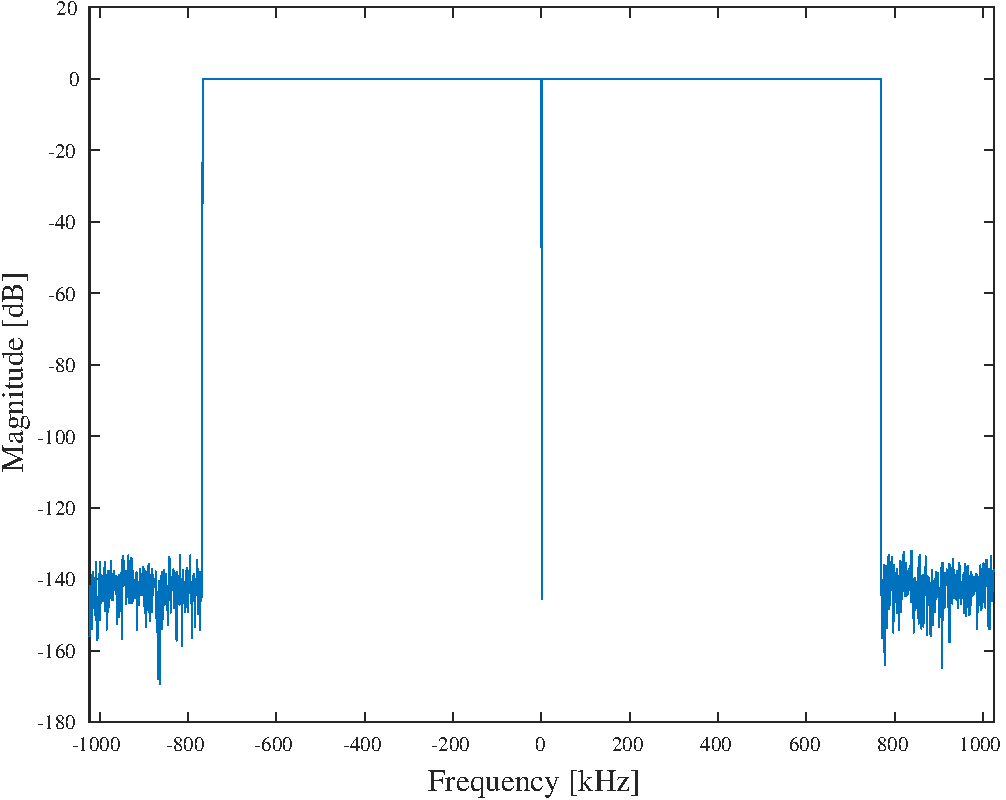
\includegraphics[width=\linewidth]{plots/ofdm-carriers-perfect.pdf}
    \caption{Perfect Data}
    \label{fig:ofdm-carriers-perfect}
  \end{subfigure}%
  ~ 
  \begin{subfigure}[t]{0.45\textwidth}
    \centering
    \captionsetup{type=figure}
    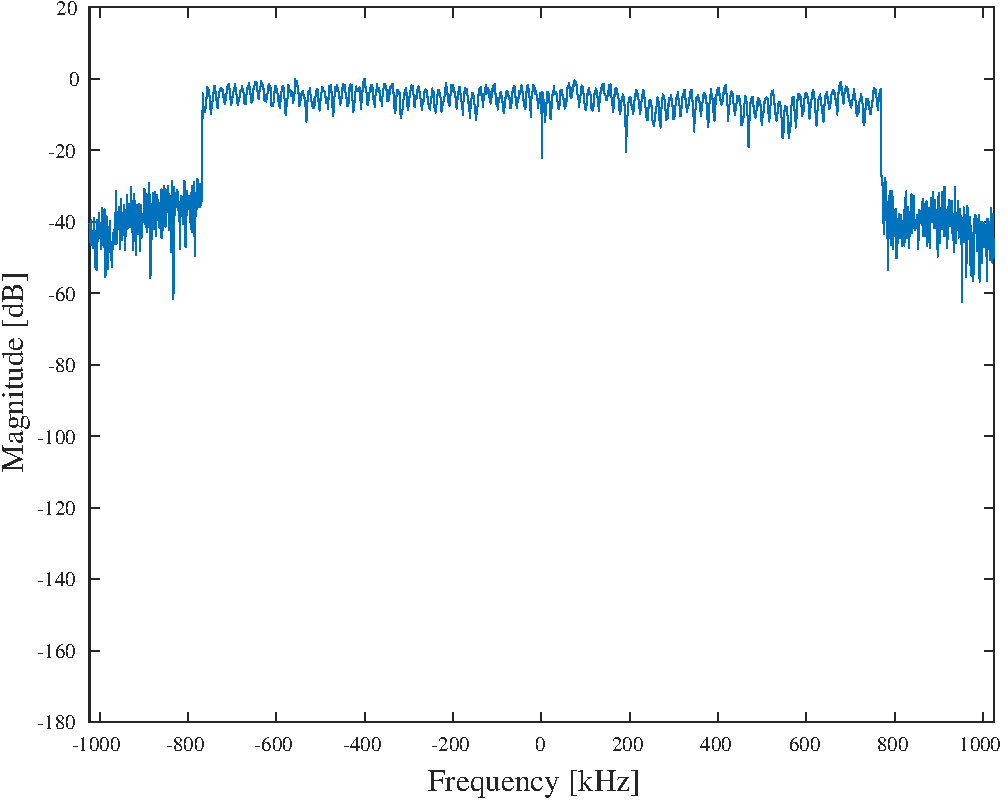
\includegraphics[width=\linewidth]{plots/ofdm-carriers-raw.pdf}
    \caption{Real-world Data}
    \label{fig:ofdm-carriers-raw}
  \end{subfigure}
  \caption{Plots showing the magnitude of the \gls{ofdm} carriers for a \gls{dab} symbol}
  \label{fig:ofdm-carriers}
\end{figure}

Recall that the \texttt{symbols\_unpack} sub-block from earlier transformed the \gls{dab} frame into \(L\) symbols of length \(T_u\). Thus, the \texttt{ofdm\_demux} sub-block was designed to receive these symbols, and output \(L\) corresponding arrays of the \(T_u\) carriers for each symbol. One can thus view the output of the function as a three-dimensional surface plot, with \(L\) successive layers of plots like those shown in Figure~\ref{fig:ofdm-carriers}. This is depicted in Figure~\ref{fig:ofdm-surface-perfect} and Figure~\ref{fig:ofdm-surface-raw} for the perfect and real-world data respectively.

\begin{figure}[htbp]
  \centering
  \captionsetup{type=figure}
  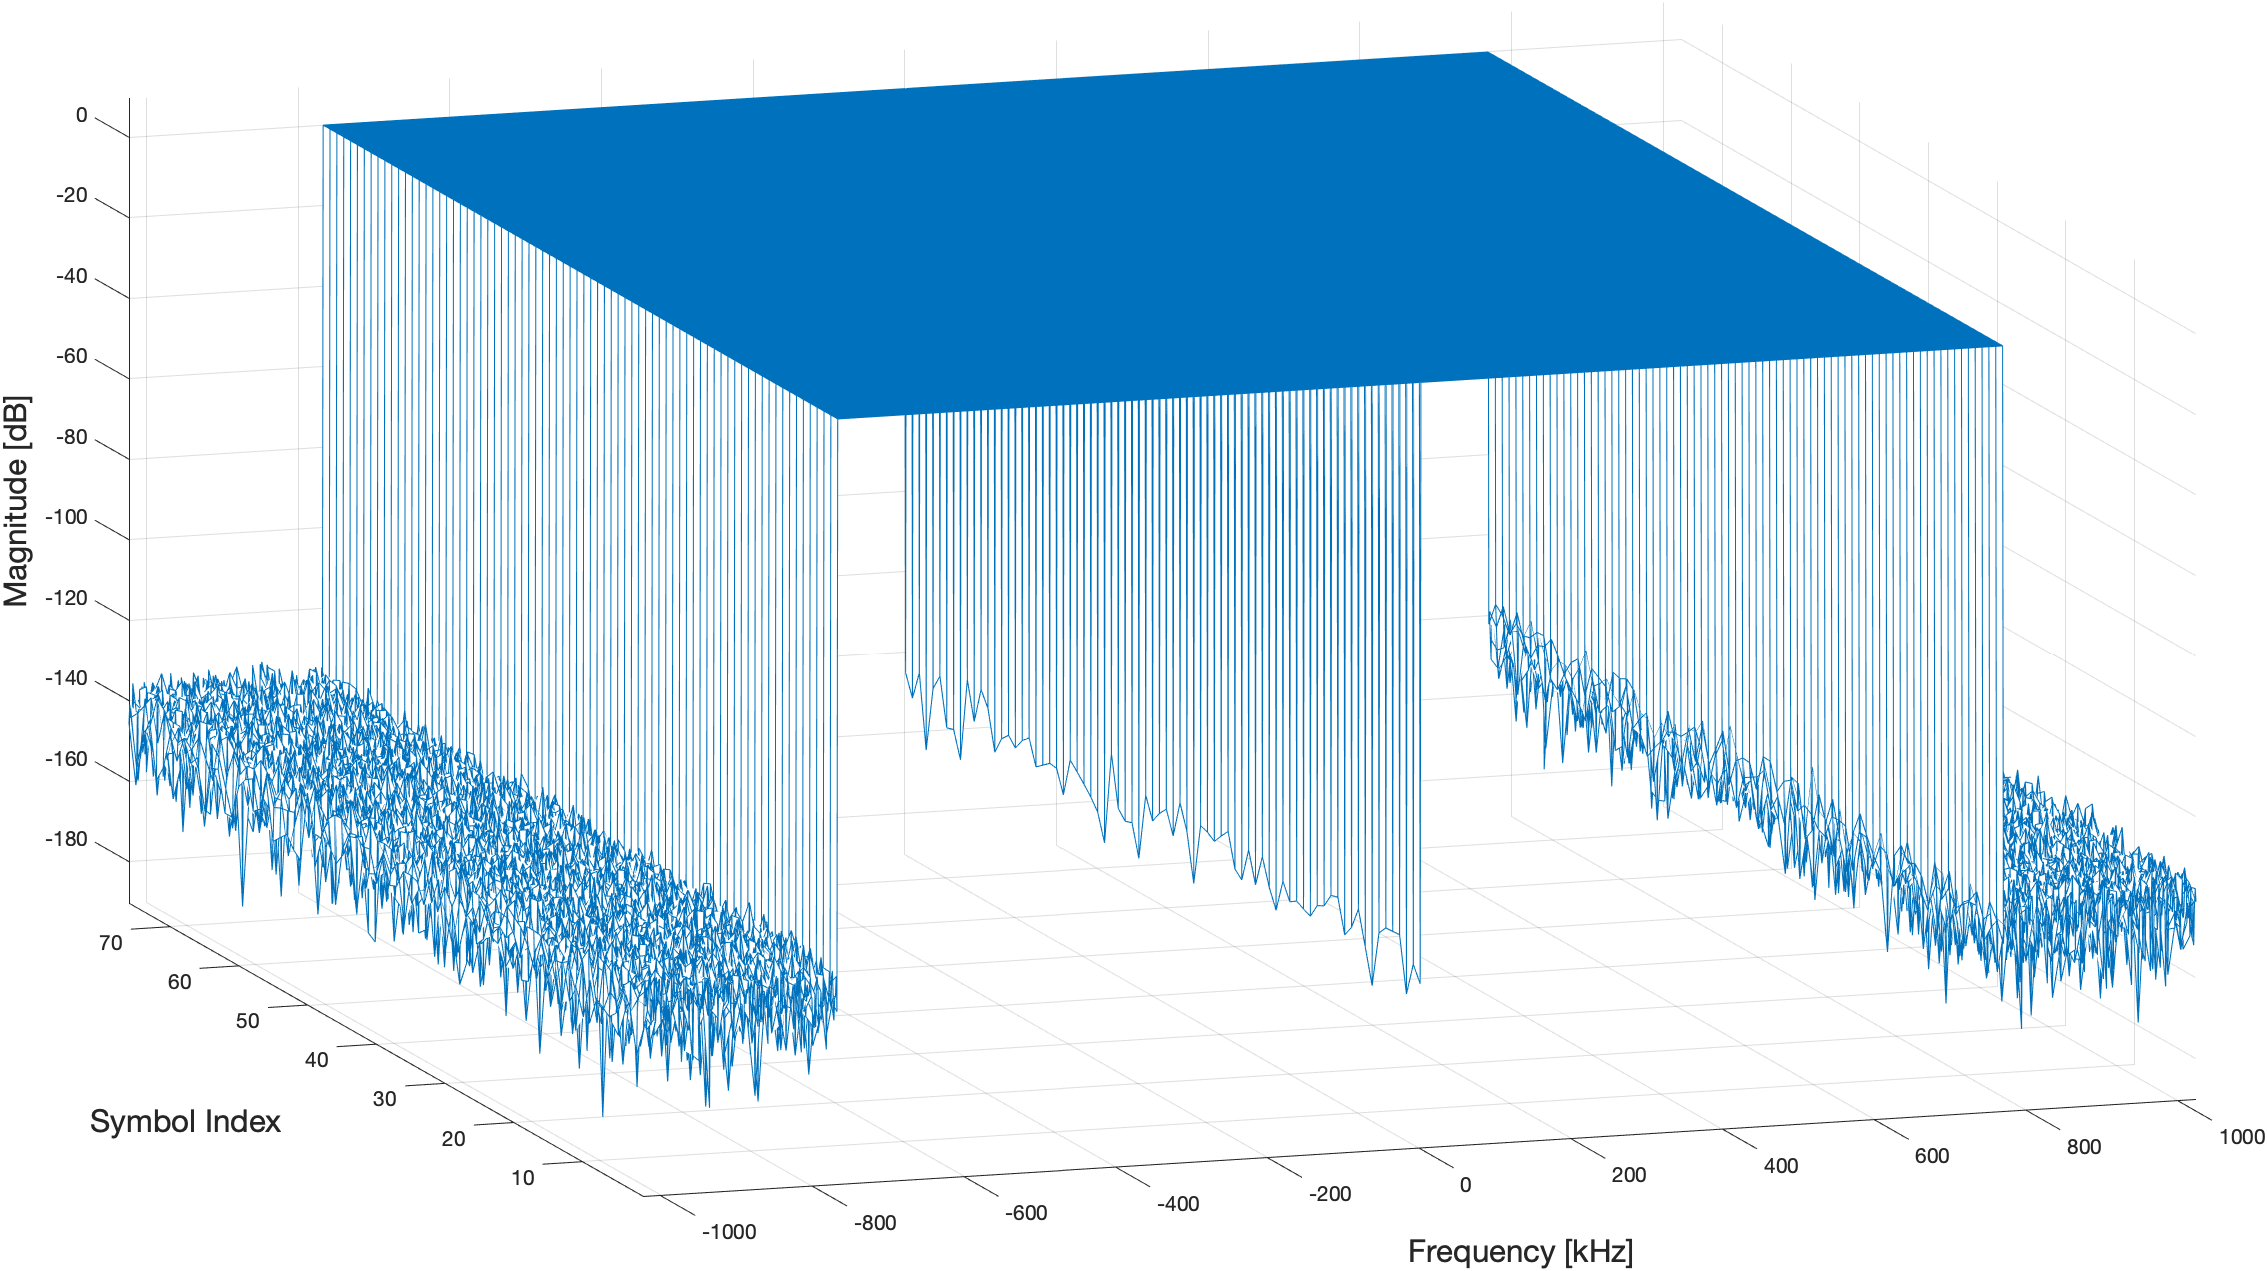
\includegraphics[width=0.7\linewidth]{plots/ofdm-surface-perfect.png}
  \caption{Surface plot of the magnitude of the \gls{ofdm} carriers for perfect data}
  \label{fig:ofdm-surface-perfect}
\end{figure}

\begin{figure}[htbp]
  \centering
  \captionsetup{type=figure}
  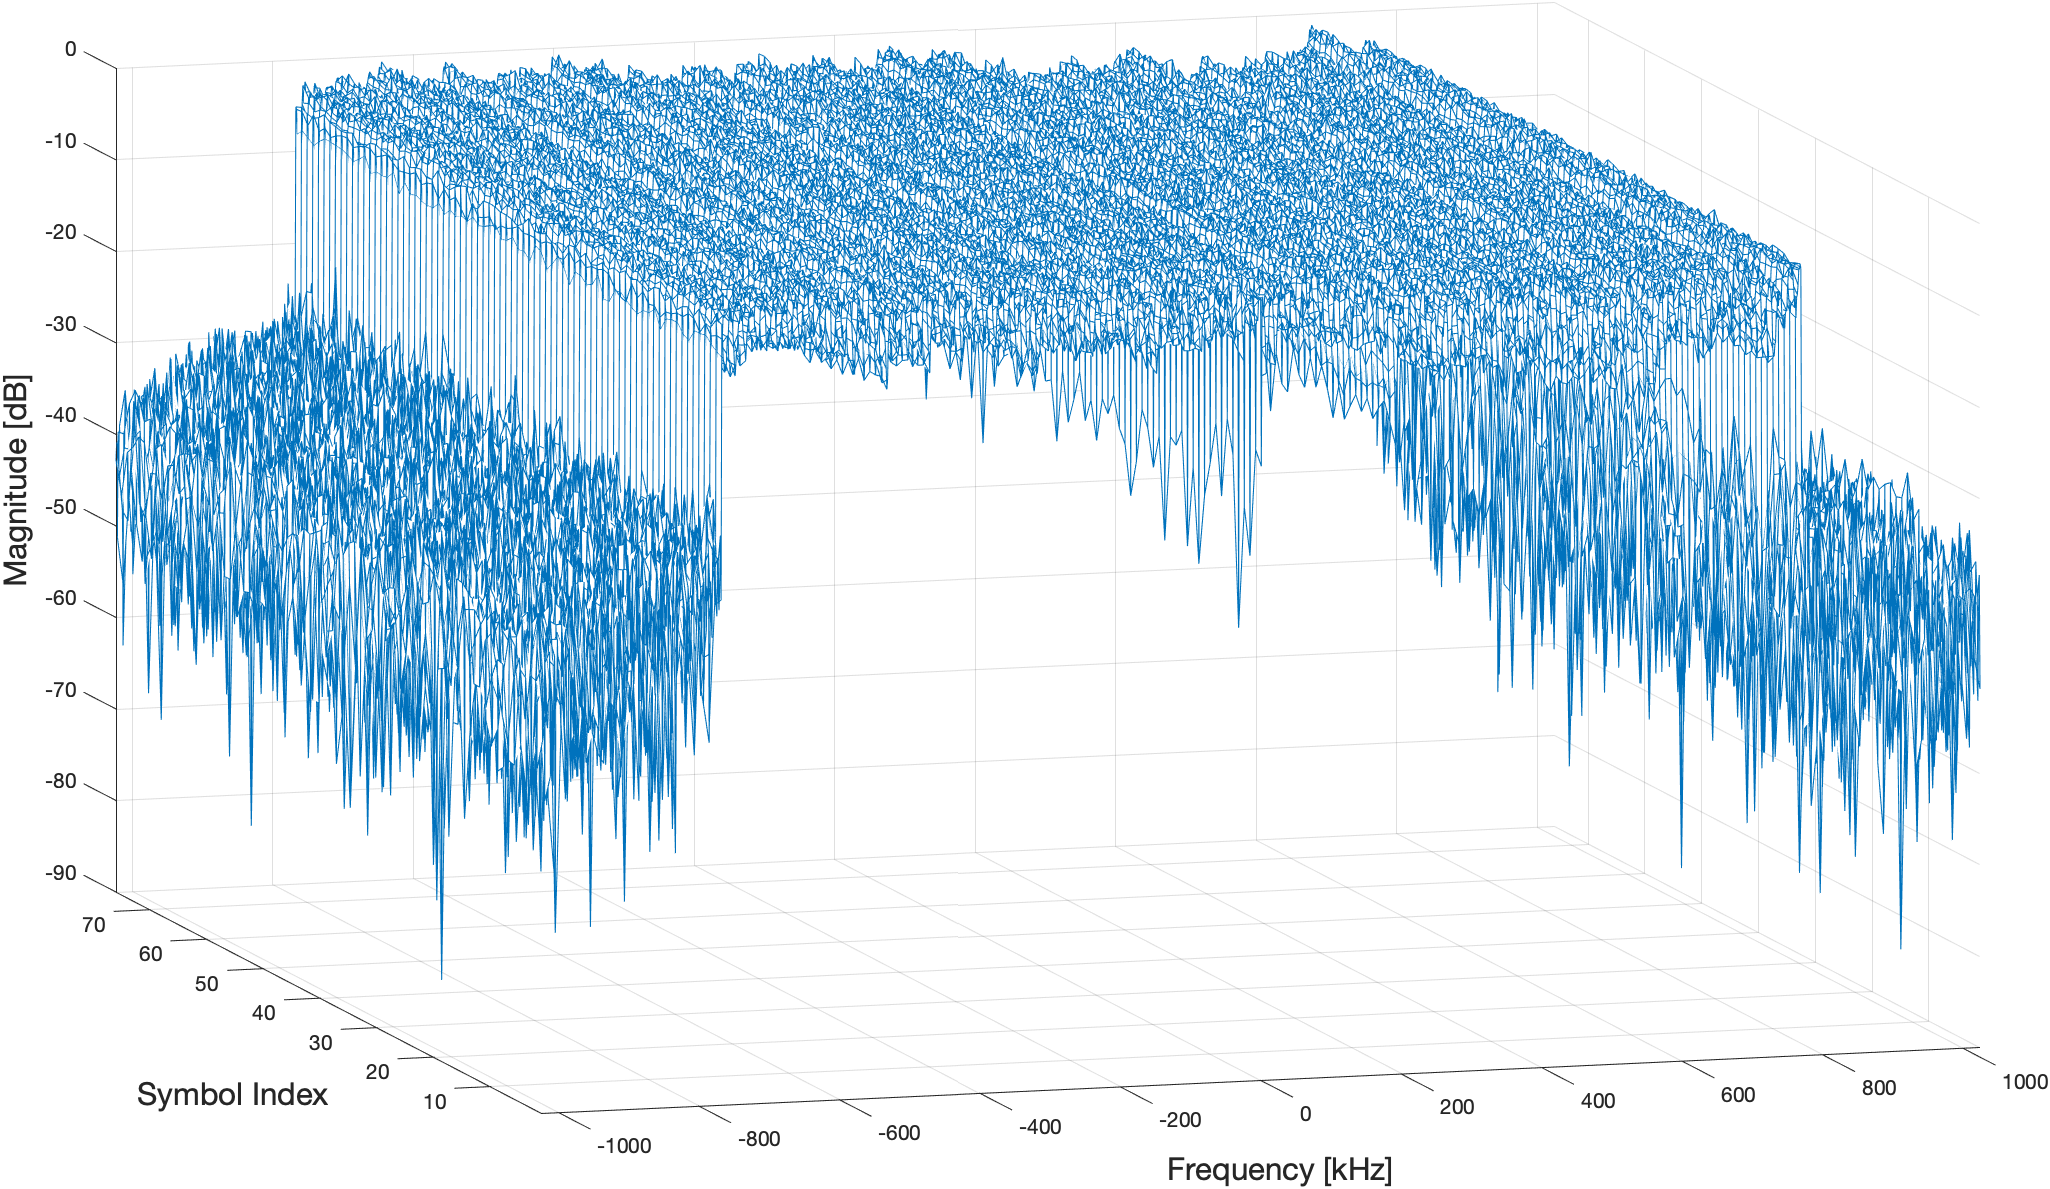
\includegraphics[width=0.7\linewidth]{plots/ofdm-surface-raw.png}
  \caption{Surface plot of the magnitude of the \gls{ofdm} carriers for real-world data}
  \label{fig:ofdm-surface-raw}
\end{figure}

A graphical summary of the \texttt{ofdm\_demux} sub-block is given in Figure~\ref{fig:ofdm_demux}, with the illustrations showing an example of real-world data.

\begin{figure}[htbp]
  \centering
  \captionsetup{type=figure}
  \def\svgwidth{\linewidth}
  {\setstretch{0.7} % Line spacing
      \input{../Images/ofdm_demux.pdf_tex}}
  \caption{Graphical summary of the \texttt{ofdm\_demux} function}
  \label{fig:ofdm_demux}
\end{figure}

\subsection{DQPSK Demapping \label{subsect:dab-proc_dqpsk-demap}}
This sub-block was designed to extract the modulating signal (the original \gls{dab} "data") from the \gls{dab} carriers. Notice that the plots of the carriers shown in the previous subsection were essentially identical from symbol to symbol, especially for the perfect data case. This is because they were showing the \emph{magnitude} of the carriers' spectra, which remains constant over time---recall that the \gls{ofdm} carriers for a \gls{dab} signal are modulated using a \(\pi/4\)-\gls{dqpsk} modulation scheme. The rectangular shape seen in the magnitude plots thus provides a good indication that the \gls{ofdm} symbols were correctly demultiplexed. From that perspective, these plots were an important graphic to consider. However, one must not forget that it is the \emph{phases} of the carriers' spectra that are modulated with actual information.

Consider the carriers from three consecutive symbols---call them \(S_{l-1}\), \(S_{l}\), and \(S_{l+1}\)---of the perfect data. The phase plots for these carriers are shown in Figure~\ref{fig:ofdm-carriers-perfect-angle}.

\begin{figure}[htbp]
  \centering
  \captionsetup{type=figure}
  \begin{subfigure}[t]{0.3\textwidth}
    \centering
    \captionsetup{type=figure}
    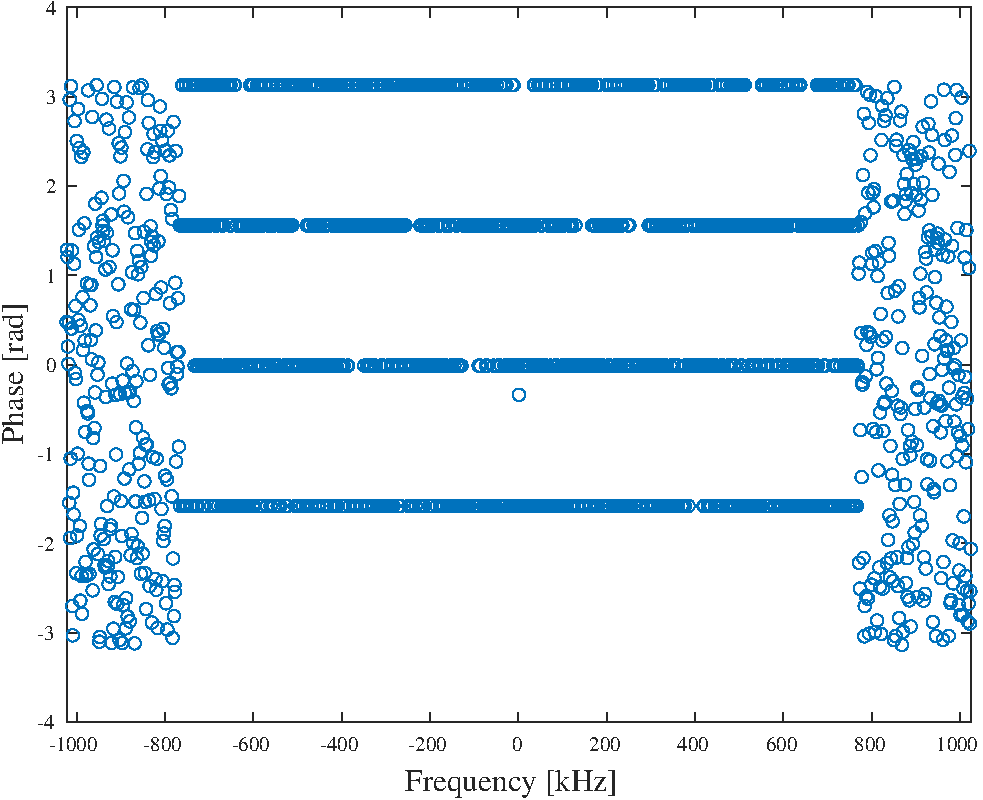
\includegraphics[width=\linewidth]{plots/ofdm-carriers-perfect-angle-1.pdf}
    \caption{\(\angle S_{l-1}\)}
    \label{fig:ofdm-carriers-perfect-angle-1}
  \end{subfigure}%
  ~ 
  \begin{subfigure}[t]{0.3\textwidth}
    \centering
    \captionsetup{type=figure}
    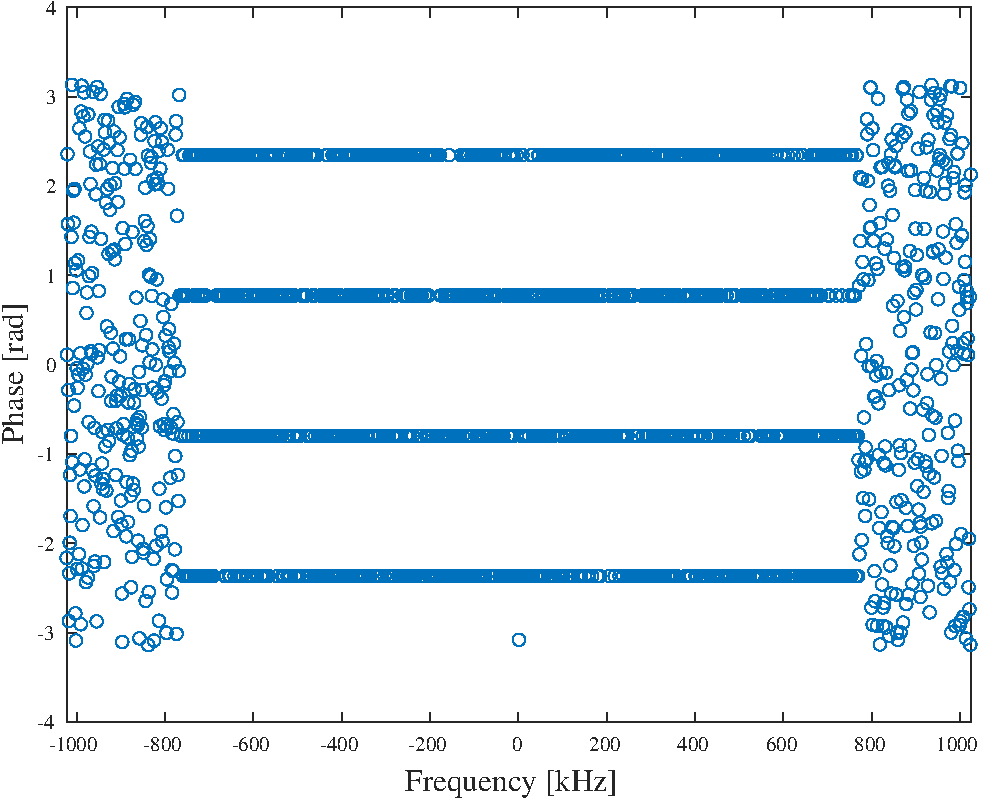
\includegraphics[width=\linewidth]{plots/ofdm-carriers-perfect-angle-2.pdf}
    \caption{\(\angle S_{l}\)}
    \label{fig:ofdm-carriers-perfect-angle-2}
  \end{subfigure}
  ~ 
  \begin{subfigure}[t]{0.3\textwidth}
    \centering
    \captionsetup{type=figure}
    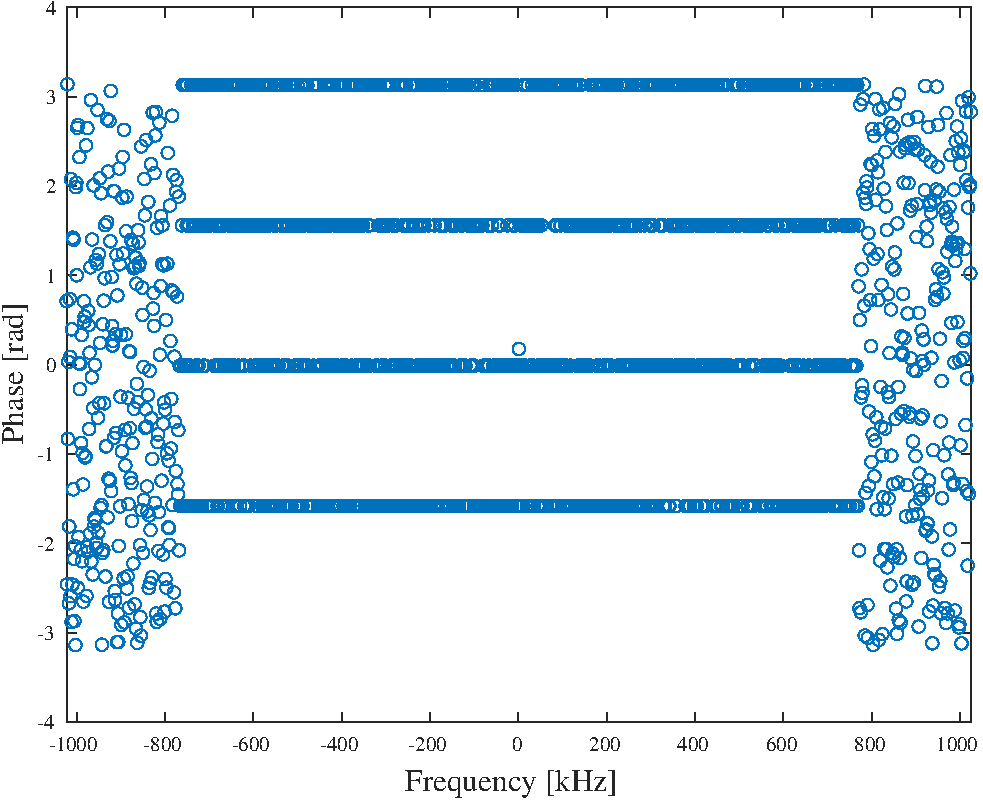
\includegraphics[width=\linewidth]{plots/ofdm-carriers-perfect-angle-3.pdf}
    \caption{\(\angle S_{l+1}\)}
    \label{fig:ofdm-carriers-perfect-angle-3}
  \end{subfigure}
  \caption{Plots showing the phase of \gls{ofdm} carriers for a three consecutive \gls{dab} symbols of perfect data}
  \label{fig:ofdm-carriers-perfect-angle}
\end{figure}

One can see that the phases of the carriers indeed changed from \(S_{l-1}\) to \(S_{l}\), and again from \(S_{l}\) to \(S_{l+1}\). The angles of the relevant carriers (the central \(K\) carriers, excluding the middle carrier) clearly correspond to one of four values, which is logical due to the \emph{quadrature} modulation scheme. Notice, though, that the possible values of these angles were different in Figure~\ref{fig:ofdm-carriers-perfect-angle-1} and Figure~\ref{fig:ofdm-carriers-perfect-angle-3}, consisting of the angles \(\{-\frac{\pi}{2}, 0, \frac{\pi}{2}, \pi\}\), compared to Figure~\ref{fig:ofdm-carriers-perfect-angle-2}, consisting of \(\{-\frac{3\pi}{4}, -\frac{\pi}{4},\frac{\pi}{4}, \frac{3\pi}{4}\}\). As explained in the previous chapter, this is because the data was \emph{differentially} modulated, with a \(\pi/4\) offset added after each symbol.

In line with this modulation scheme, the process of extracting the \gls{dab} data from the carriers involved considering the phase difference between consecutive symbols, with the first symbol, the \gls{prs}, used as a reference for subsequent symbols (hence its name). This process was termed "demapping" the \gls{dqpsk} data. Since the data was demapped using the difference of two symbols, a given set of \(L\)~symbols mapped to \((L-1)\) streams of \gls{dab} data.

Consider the extraction of the data for an arbitrary index, \((l-1)\), call this data \(D_{l-1}\), from the symbols \(S_{l-1}\) and \(S_{l}\). Using a simple complex relation,
\begin{align}
  D_{l-1} &= \angle S_{l} - \angle S_{l-1}\\
          &= \angle\left(\frac{S_{l}}{S_{l-1}}\right)
\end{align}

This process can be easily be achieved in software---for example, using the simple code given in Listing~\ref{code:dqpsk_demap}. To avoid unnecessary division computation, this calculation was only done for the relevant carriers, indexed in MATLAB using the variable called \texttt{mask}. Here, \texttt{dab\_carriers(n,:)} refers to \(S_n\), and \texttt{dab\_data\_raw(n,:)} refers to \(D_n\).

\begin{lstlisting}[caption={MATLAB code for demapping \gls{dab} carriers into \gls{dqpsk} data},label={code:dqpsk_demap}]
dab_data_raw(l-1,mask) = dab_carriers(l,mask) ./ dab_carriers(l-1,mask);
\end{lstlisting}

It was also useful to view the angles of the carrier waves on a complex plane. Though this perspective does not show the progression of the angles over time, nor the relationships between the angles of the carriers in nearby frequency regions, it does show the spread of the data. Consider once again the carriers from two symbols, \(S_{l-1}\) and \(S_{l}\), of the perfect data. These are shown plotted on the complex plane in Figure~\ref{fig:dqpsk_demap_perfect-1} and Figure~\ref{fig:dqpsk_demap_perfect-2}. These plots essentially show the same information as Figure~\ref{fig:ofdm-carriers-perfect-angle-1} and Figure~\ref{fig:ofdm-carriers-perfect-angle-2}. Figure~\ref{fig:dqpsk_demap_perfect-2over1} then shows \(D_{l-1}\), which is the quotient of \(S_{l}\) by \(S_{l-1}\). Because this data is perfect, the angles are perfectly assigned to one of the four differential values.

\begin{figure}[htbp]
  \centering
  \captionsetup{type=figure}
  \begin{subfigure}[t]{0.3\textwidth}
    \centering
    \captionsetup{type=figure}
    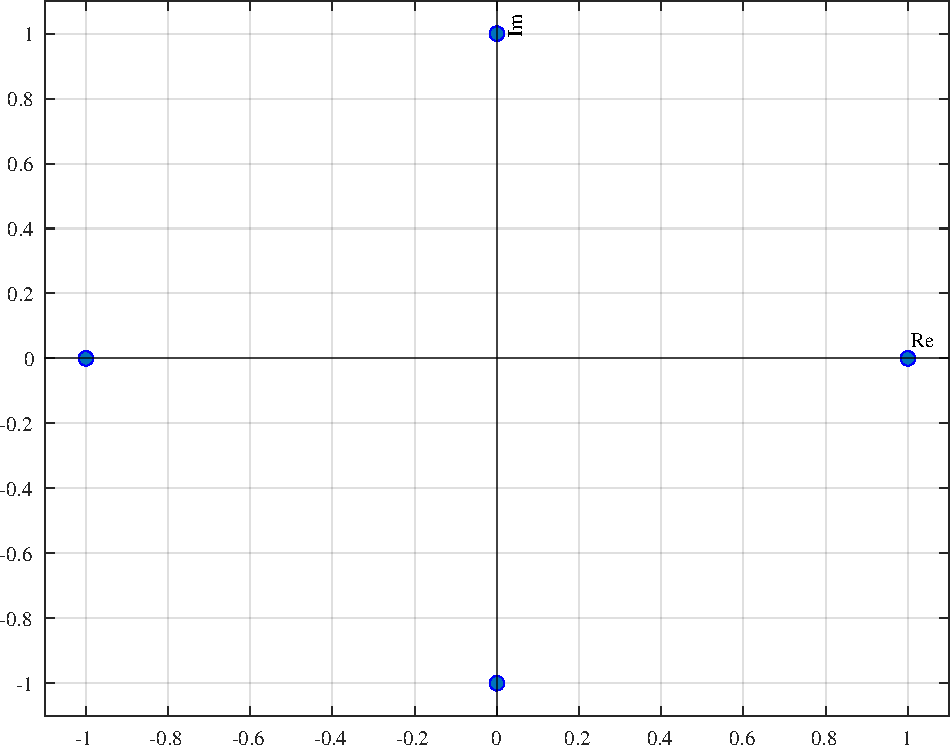
\includegraphics[width=\linewidth]{plots/dqpsk_demap_perfect-1.pdf}
    \caption{\(S_{l-1}\)}
    \label{fig:dqpsk_demap_perfect-1}
  \end{subfigure}%
  ~ 
  \begin{subfigure}[t]{0.3\textwidth}
    \centering
    \captionsetup{type=figure}
    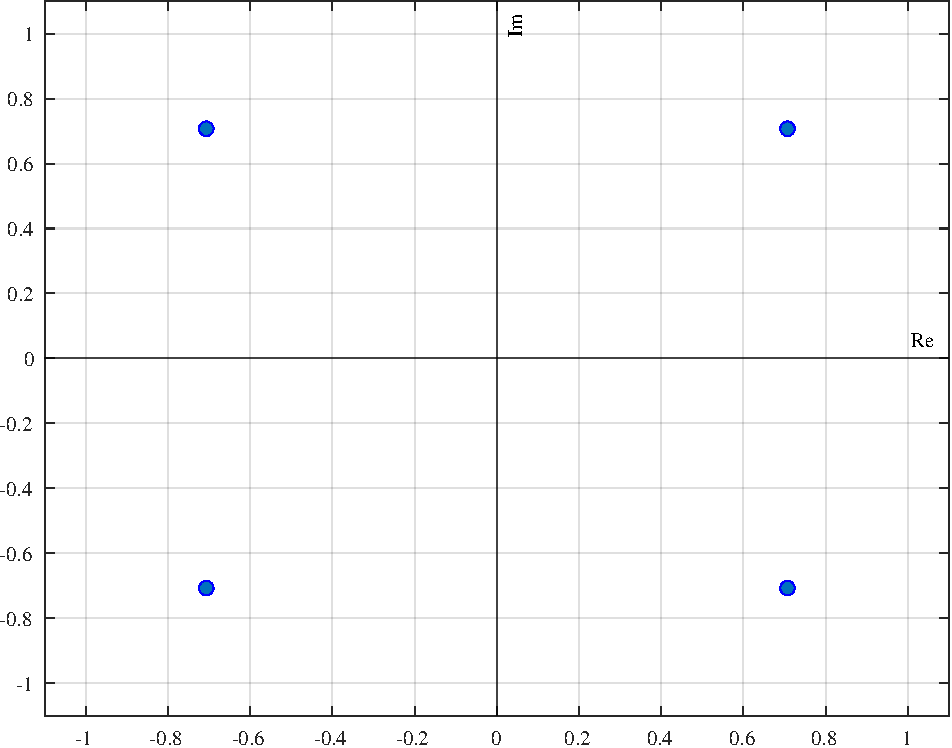
\includegraphics[width=\linewidth]{plots/dqpsk_demap_perfect-2.pdf}
    \caption{\(S_{l}\)}
    \label{fig:dqpsk_demap_perfect-2}
  \end{subfigure}
  ~ 
  \begin{subfigure}[t]{0.3\textwidth}
    \centering
    \captionsetup{type=figure}
    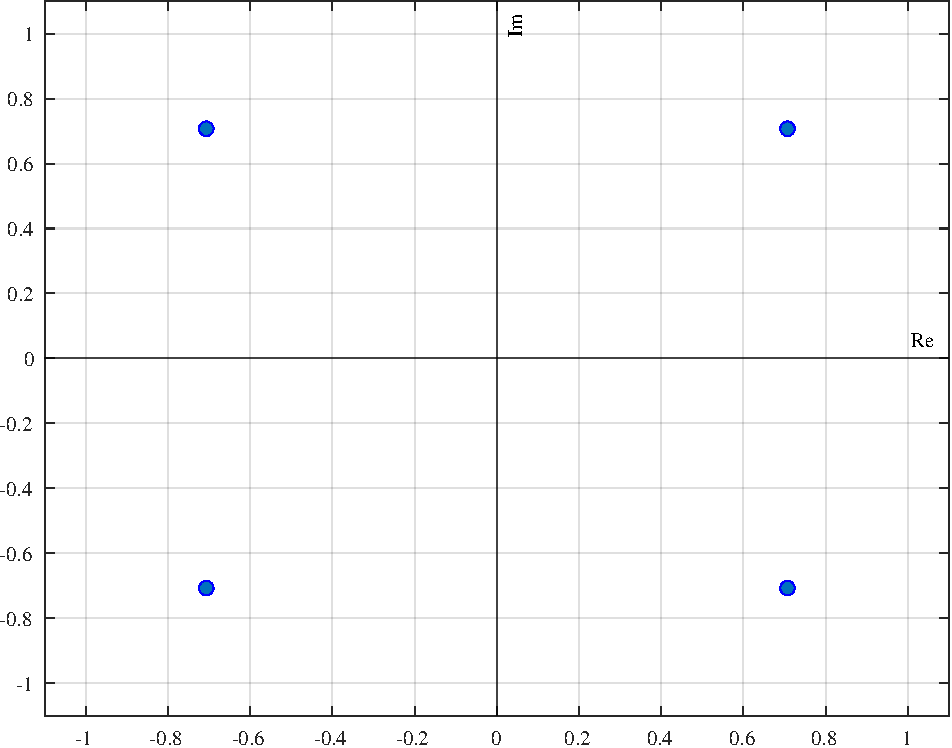
\includegraphics[width=\linewidth]{plots/dqpsk_demap_perfect-2over1.pdf}
    \caption{\(D_{l-1} = S_{l}/S_{l-1}\)}
    \label{fig:dqpsk_demap_perfect-2over1}
  \end{subfigure}
  \caption{Plots shown on the complex plane of various data derived from a perfect \gls{dab} signal.}
  \label{fig:dqpsk_demap_perfect}
\end{figure}

Though the plots in Figure~\ref{fig:dqpsk_demap_perfect} are correct, they do not demonstrate the power of \gls{dqpsk} clearly. One may wonder whether simple \gls{qpsk} modulation would be good enough, given how neat the angles were shown to be. Therefore, it is important to consider some real-world signals. Firstly, consider Figure~\ref{fig:dqpsk_demap_rtl}, which shows the same plots as before, but for an actual, recorded \gls{dab} signal.

\begin{figure}[htbp]
  \centering
  \captionsetup{type=figure}
  \begin{subfigure}[t]{0.3\textwidth}
    \centering
    \captionsetup{type=figure}
    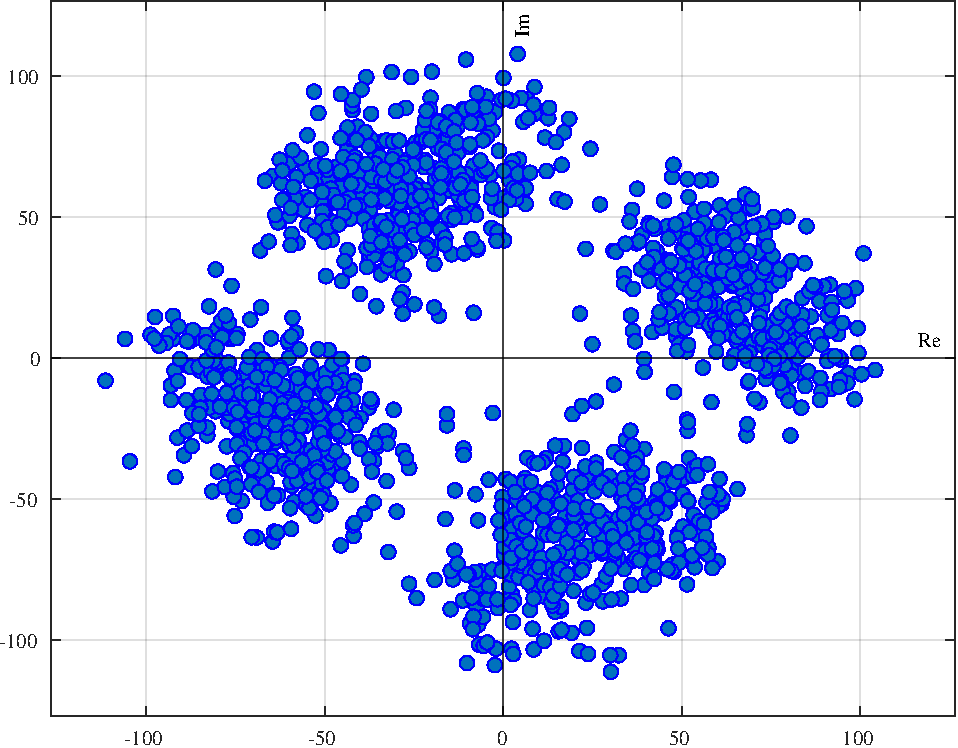
\includegraphics[width=\linewidth]{plots/dqpsk_demap_rtl-1.pdf}
    \caption{\(S_{l-1}\)}
    \label{fig:dqpsk_demap_rtl-1}
  \end{subfigure}%
  ~ 
  \begin{subfigure}[t]{0.3\textwidth}
    \centering
    \captionsetup{type=figure}
    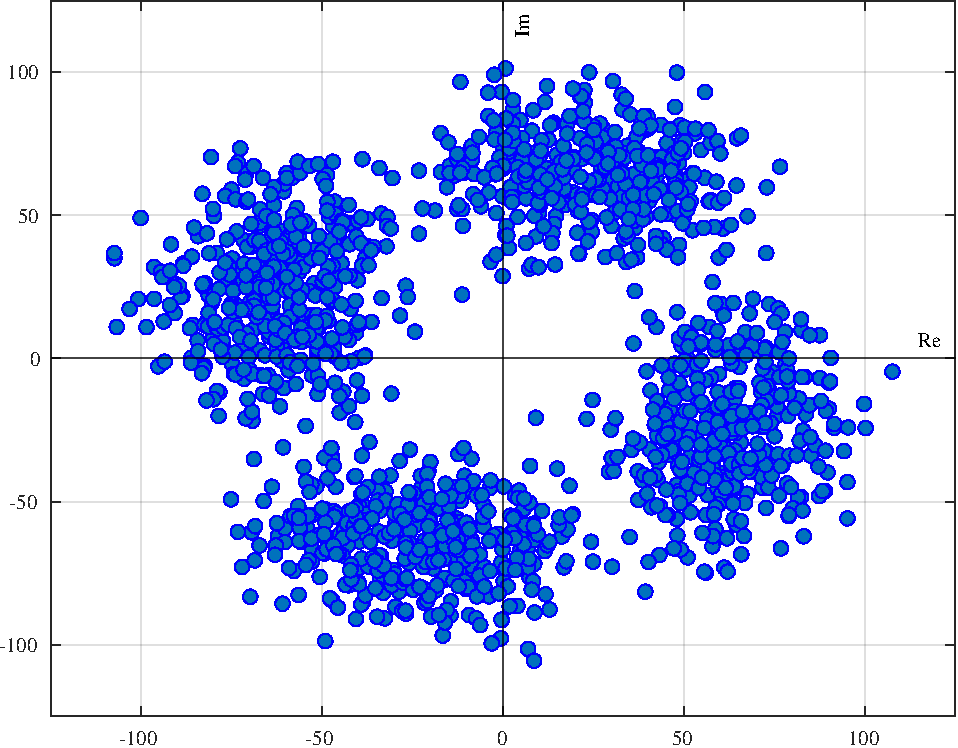
\includegraphics[width=\linewidth]{plots/dqpsk_demap_rtl-2.pdf}
    \caption{\(S_{l}\)}
    \label{fig:dqpsk_demap_rtl-2}
  \end{subfigure}
  ~ 
  \begin{subfigure}[t]{0.3\textwidth}
    \centering
    \captionsetup{type=figure}
    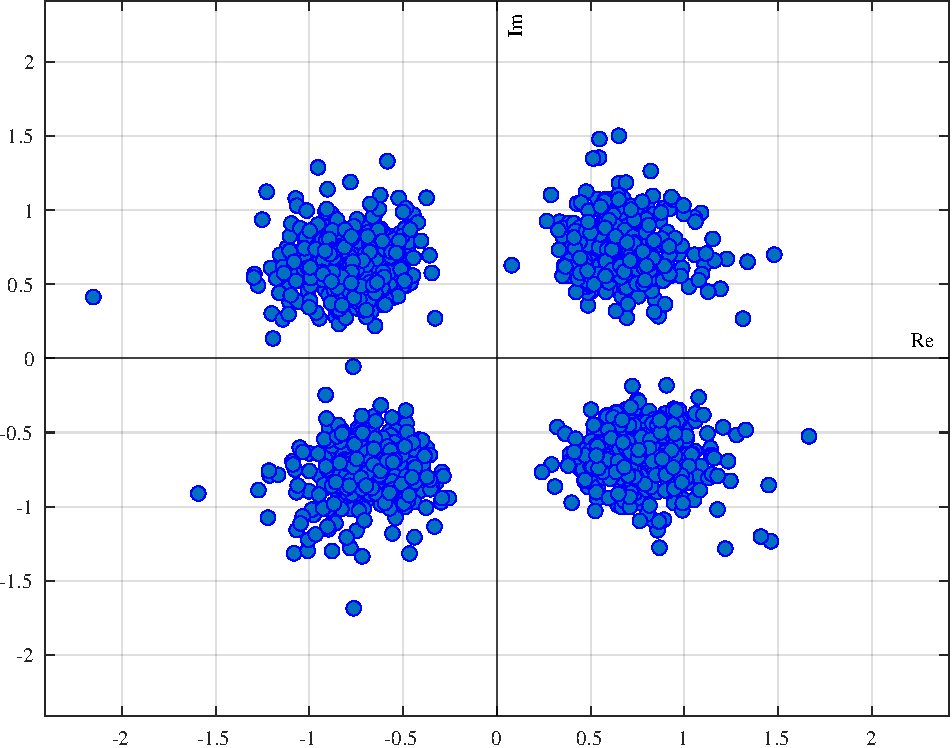
\includegraphics[width=\linewidth]{plots/dqpsk_demap_rtl-2over1.pdf}
    \caption{\(D_{l-1} = S_{l}/S_{l-1}\)}
    \label{fig:dqpsk_demap_rtl-2over1}
  \end{subfigure}
  \caption{Plots shown on the complex plane of various data derived from a real-world \gls{dab} signal.}
  \label{fig:dqpsk_demap_rtl}
\end{figure}

Notice how the spread of the angles in Figure~\ref{fig:dqpsk_demap_rtl-1} and Figure~\ref{fig:dqpsk_demap_rtl-2} is far worse than seen previously with the perfect data. Though one can see four broad groups of data, the precise decision boundary between these groups is uncertain. In contrast, see how much more distinct these groups become in Figure~\ref{fig:dqpsk_demap_rtl-2over1}, thanks to the differential modulation. Indeed, there is still spreading, but the decision boundary is far clearer.

Consider an even more extreme example, from some poor-quality \gls{dab} data. Figure~\ref{fig:dqpsk_demap_raw-1} and Figure~\ref{fig:dqpsk_demap_raw-2} show the angles of the carriers for the two symbols---notice how there are no distinct groupings whatsoever. In fact, the data seems to be randomly spread. Nonetheless, by looking at the phase-difference between the two symbols, the four groups become far more coherent, as shown in Figure~\ref{fig:dqpsk_demap_raw-2over1}. Granted, there seems to be a phase offset in the differences of around \(\frac{\pi}{8}\) radians, but the \gls{dqpsk} values are nonetheless distinct.

\begin{figure}[htbp]
  \centering
  \captionsetup{type=figure}
  \begin{subfigure}[t]{0.3\textwidth}
    \centering
    \captionsetup{type=figure}
    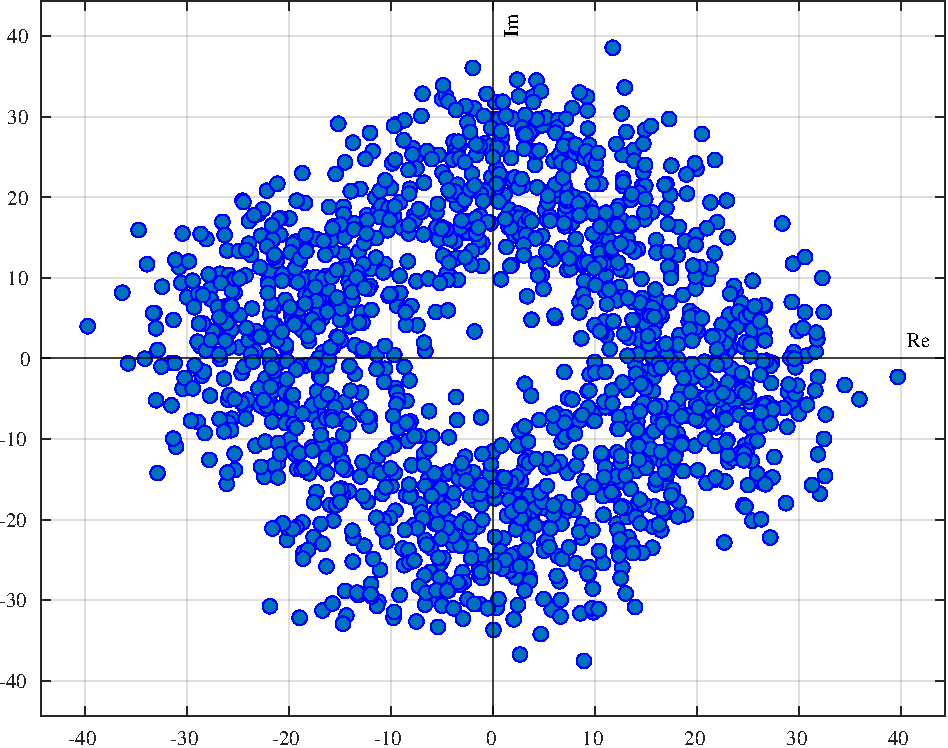
\includegraphics[width=\linewidth]{plots/dqpsk_demap_raw-1.pdf}
    \caption{\(S_{l-1}\)}
    \label{fig:dqpsk_demap_raw-1}
  \end{subfigure}%
  ~ 
  \begin{subfigure}[t]{0.3\textwidth}
    \centering
    \captionsetup{type=figure}
    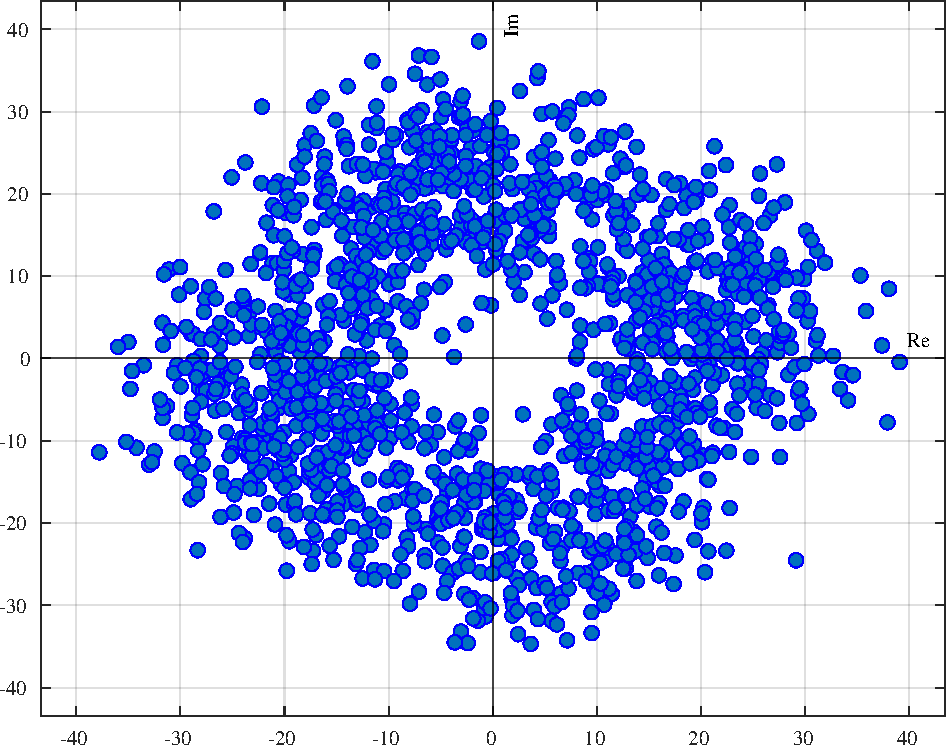
\includegraphics[width=\linewidth]{plots/dqpsk_demap_raw-2.pdf}
    \caption{\(S_{l}\)}
    \label{fig:dqpsk_demap_raw-2}
  \end{subfigure}
  ~ 
  \begin{subfigure}[t]{0.3\textwidth}
    \centering
    \captionsetup{type=figure}
    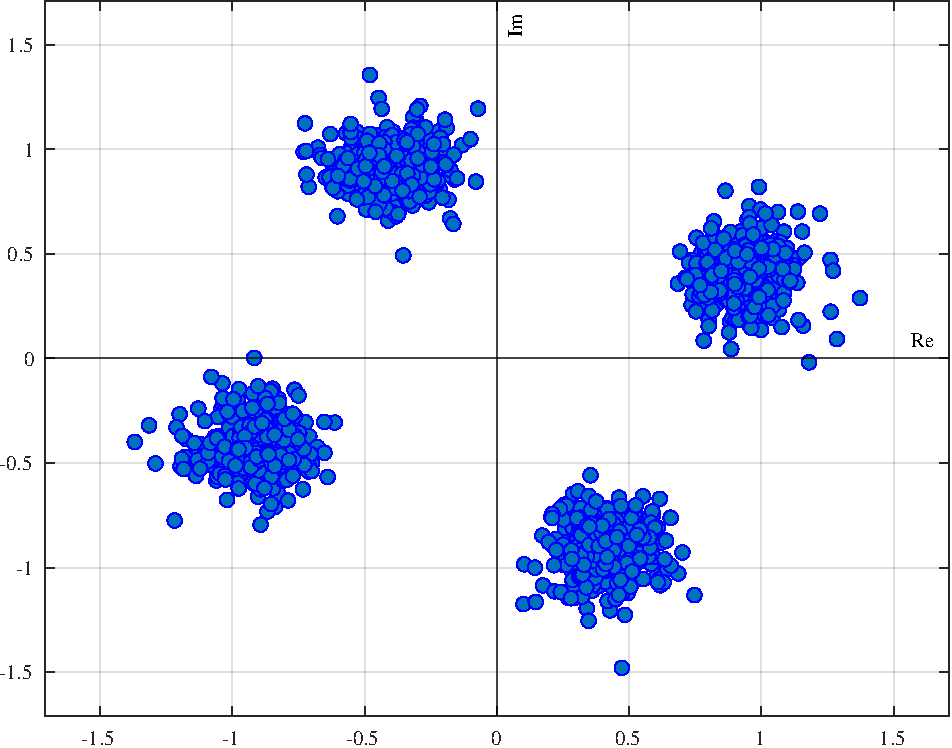
\includegraphics[width=\linewidth]{plots/dqpsk_demap_raw-2over1.pdf}
    \caption{\(D_{l-1} = S_{l}/S_{l-1}\)}
    \label{fig:dqpsk_demap_raw-2over1}
  \end{subfigure}
  \caption{Plots shown on the complex plane of various data derived from a poor-quality \gls{dab} signal.}
  \label{fig:dqpsk_demap_raw}
\end{figure}

In summary, this block "demapped" the \gls{dqpsk}-modulated data from the \gls{dab} carriers by calculating the phase-difference between the carriers from consecutive symbols. This was done for all of the \(L\) sets of carriers provided, thus producing \((L-1)\) sets of data. This functionality is shown graphically in Figure~\ref{fig:dqpsk_demap}.

\begin{figure}[htbp]
  \centering
  \captionsetup{type=figure}
  \def\svgwidth{\linewidth}
  {\setstretch{0.7} % Line spacing
      \input{../Images/dqpsk_demap.pdf_tex}}
      \caption{Graphical summary of the \texttt{dqpsk\_demap} function.}
  \label{fig:dqpsk_demap}
\end{figure}

\subsection{Frequency Deinterleaving \label{subsect:dab-proc_freq-deinterleave}}
This sub-block, termed \texttt{freq\_deinterleave}, was created to receive \((L-1)\) interleaved sets of \gls{dqpsk}-demodulated data, and return the same data but deinterleaved according to a given map. In the previous chapter, the problem of frequency-selective fading was discussed, along with the \gls{dab} standard's mitigation strategy of interleaving the \gls{ofdm} carriers in a particular way. The precise motivation and details of the specific map used for interleaving are given in \gls{etsi}'s document in~\cite{dabstandard}. Note that the input data, the output of the \texttt{dqpsk\_demap} block, included all \(T_u\) carriers, including those which were outside the band of the central \(K\) carriers. In performing the frequency deinterleaving process, this function also removed the out-of-band carriers, leaving only the \(K\) relevant carriers.

For convenience, a helper function was written in MATLAB, called \texttt{build\_interleave\_map()}, which returned an array mapping the \(K\) indices of an array to \(K\) corresponding interleaved indices. Importantly, note that the mapping used differs for each of the four \gls{dab} transmission modes. Since this project was designed using Mode I signals, the code was implemented with Mode I's interleaving map, and with \(K = 1536\). The full code for this function is provided in Appendix (?). Future work should be done to enable this functionality for all four \gls{dab} modes.

Once the interleave map was created, deinterleaving the frequency components was trivial, as it simply entailed indexing the MATLAB matrices appropriately. The \texttt{freq\_deinterleave} function is given in Listing~\ref{code:freq_deinterleave}. Notice that this code is independent of the \gls{dab} mode used, relying only on a generic interleaving map.

\begin{lstlisting}[caption={MATLAB code for the frequency deinterleaving functionality.},label={code:freq_deinterleave}]
function dab_data_deinterleaved = freq_deinterleave(dab_data_raw, interleave_map)
  dab_data_deinterleaved = dab_data_raw(:,interleave_map); % Use interleave map for indexing
end
\end{lstlisting}

When visualized, the deinterleaving of the frequency components is not particularly insightful, as the large number of sub-carriers involved can make the plots messy. Consider, for example, the plot of the carriers' phases for a real-world \gls{dab} symbol in Figure~\ref{fig:freq_deinterleave_plot}.

\begin{figure}[htbp]
  \centering
  \captionsetup{type=figure}
  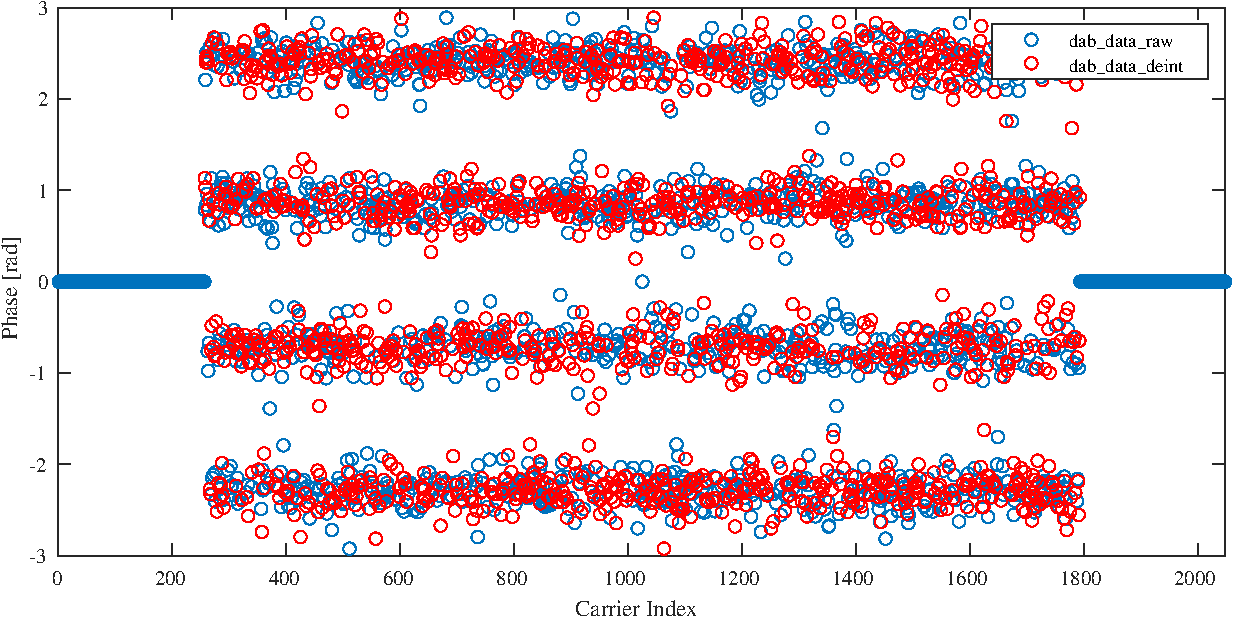
\includegraphics[width=0.9\linewidth]{plots/freq_deinterleave_plot.pdf}
  \caption{Phase plot for the carriers of a real-world \gls{dab} symbol, before and after frequency deinterleaving.}
  \label{fig:freq_deinterleave_plot}
\end{figure}

Even the plot of the interleaving map for Mode I looks somewhat arbitrary, as seen in Figure~\ref{fig:interleave_map}.
%This makes sense, as the \gls{dab} standard intended to distribute the carriers as (randomly ...) as possible.

\begin{figure}[htbp]
  \centering
  \captionsetup{type=figure}
  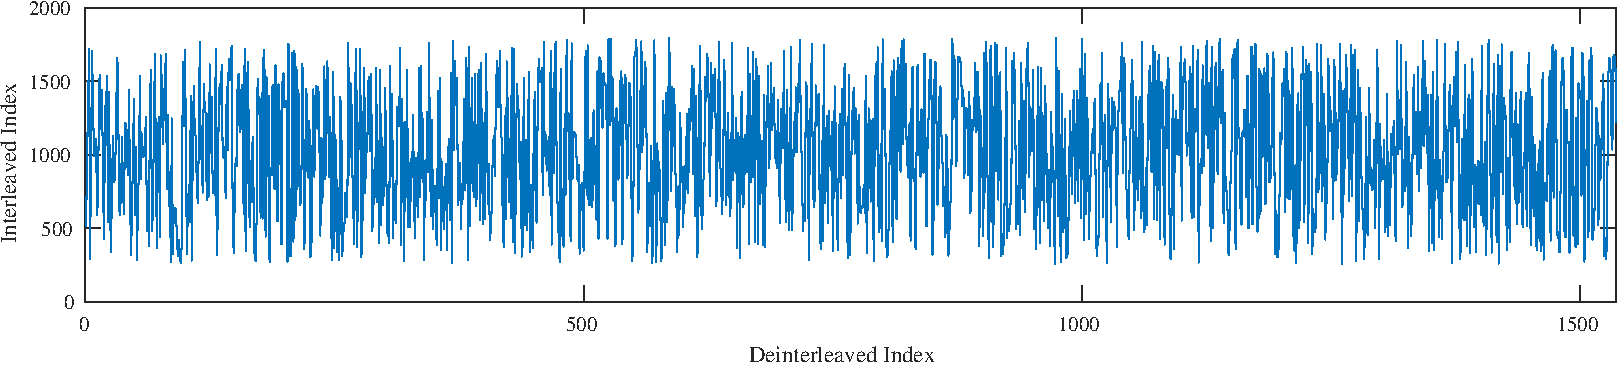
\includegraphics[width=\linewidth]{plots/interleave_map.pdf}
  \caption{Interleave map for \gls{dab} Transmission Mode I.}
  \label{fig:interleave_map}
\end{figure}

%Nevertheless, since the out-of-band carriers---which were set to a phase of 0 in the \texttt{dqpsk\_demap} sub-block---were removed, one will no longer see a \((0,0)\) point on the complex plane.
Nonetheless, the graphical summary for the \texttt{freq\_deinterleave} function is given in Figure~\ref{fig:freq_deinterleave}.

\begin{figure}[htbp]
  \centering
  \captionsetup{type=figure}
  \def\svgwidth{\linewidth}
  {\setstretch{0.7} % Line spacing
      \input{../Images/freq_deinterleave.pdf_tex}}
  \caption{Graphical summary of the \texttt{freq\_deinterleave} function.}
  \label{fig:freq_deinterleave}
\end{figure}

\subsection{DQPSK Snapping \label{subsect:dab-proc_dqpsk-snap}}
As seen in Figure~\ref{fig:dqpsk_demap_rtl-2over1} and Figure~\ref{fig:dqpsk_demap_raw-2over1}, the \texttt{dqpsk\_demap} sub-block did well to distinguish four groups of differential phase values from the \gls{ofdm} carriers, despite being provided with input data that was fairly spread-out. Nonetheless, the spread of the data within these groups was still a problem---the groups each needed to be assigned to one of four values. Fortunately, provided one can assume that the original, transmitted signal was modulated correctly according the \gls{dab} standard in~\cite{dabstandard}, the four possible \emph{correct} phase-difference angles were known \emph{a priori}. Those being, \(\{-\frac{3\pi}{4}, -\frac{\pi}{4},\frac{\pi}{4}, \frac{3\pi}{4}\}\). Since only the phase is modulated, the magnitude of the carriers should remain constant from symbol to symbol, and thus the magnitude of the complex ratio between any two symbols should be 1. In rectangular co-ordinates, then, the four possible points correspond to the values, \(\pm \frac{1}{\sqrt{2}} \pm j\frac{1}{\sqrt{2}}\).

The easiest way to correct the spread of the \gls{dqpsk} symbols was to re-assign them with the value that was closest to them out of the four possible points. Due to their angles, the four points fall exactly in the centre of each of the four quadrants respectively. Thus, if a given point was in quadrant \(X\), it was guaranteed to be closest to the correct \gls{dqpsk} point in that quadrant. Of course, this method of correcting real-world \gls{dab} data was not perfect, in that it did not apply any robust error-correction techniques to the data, and it likely assigned some edge cases incorrectly. Nonetheless, it was a quick and easy way to extract meaningful \gls{dqpsk} data. This process was termed "snapping", as it snapped given points to their closest possible values. Figure~\ref{fig:dqpsk_snap_rtl} shows an example symbol from real-world data (perfect data need not be snapped, as it is perfect already), where the four groups from the \gls{dqpsk}-demapping fell within the four quadrants on a complex plane. Any given point, then, was simply snapped to the value for that quadrant. The groupings are shown by different colours, and the snapped values are shown by the large blue crosses.

\begin{figure}[htbp]
  \centering
  \captionsetup{type=figure}
  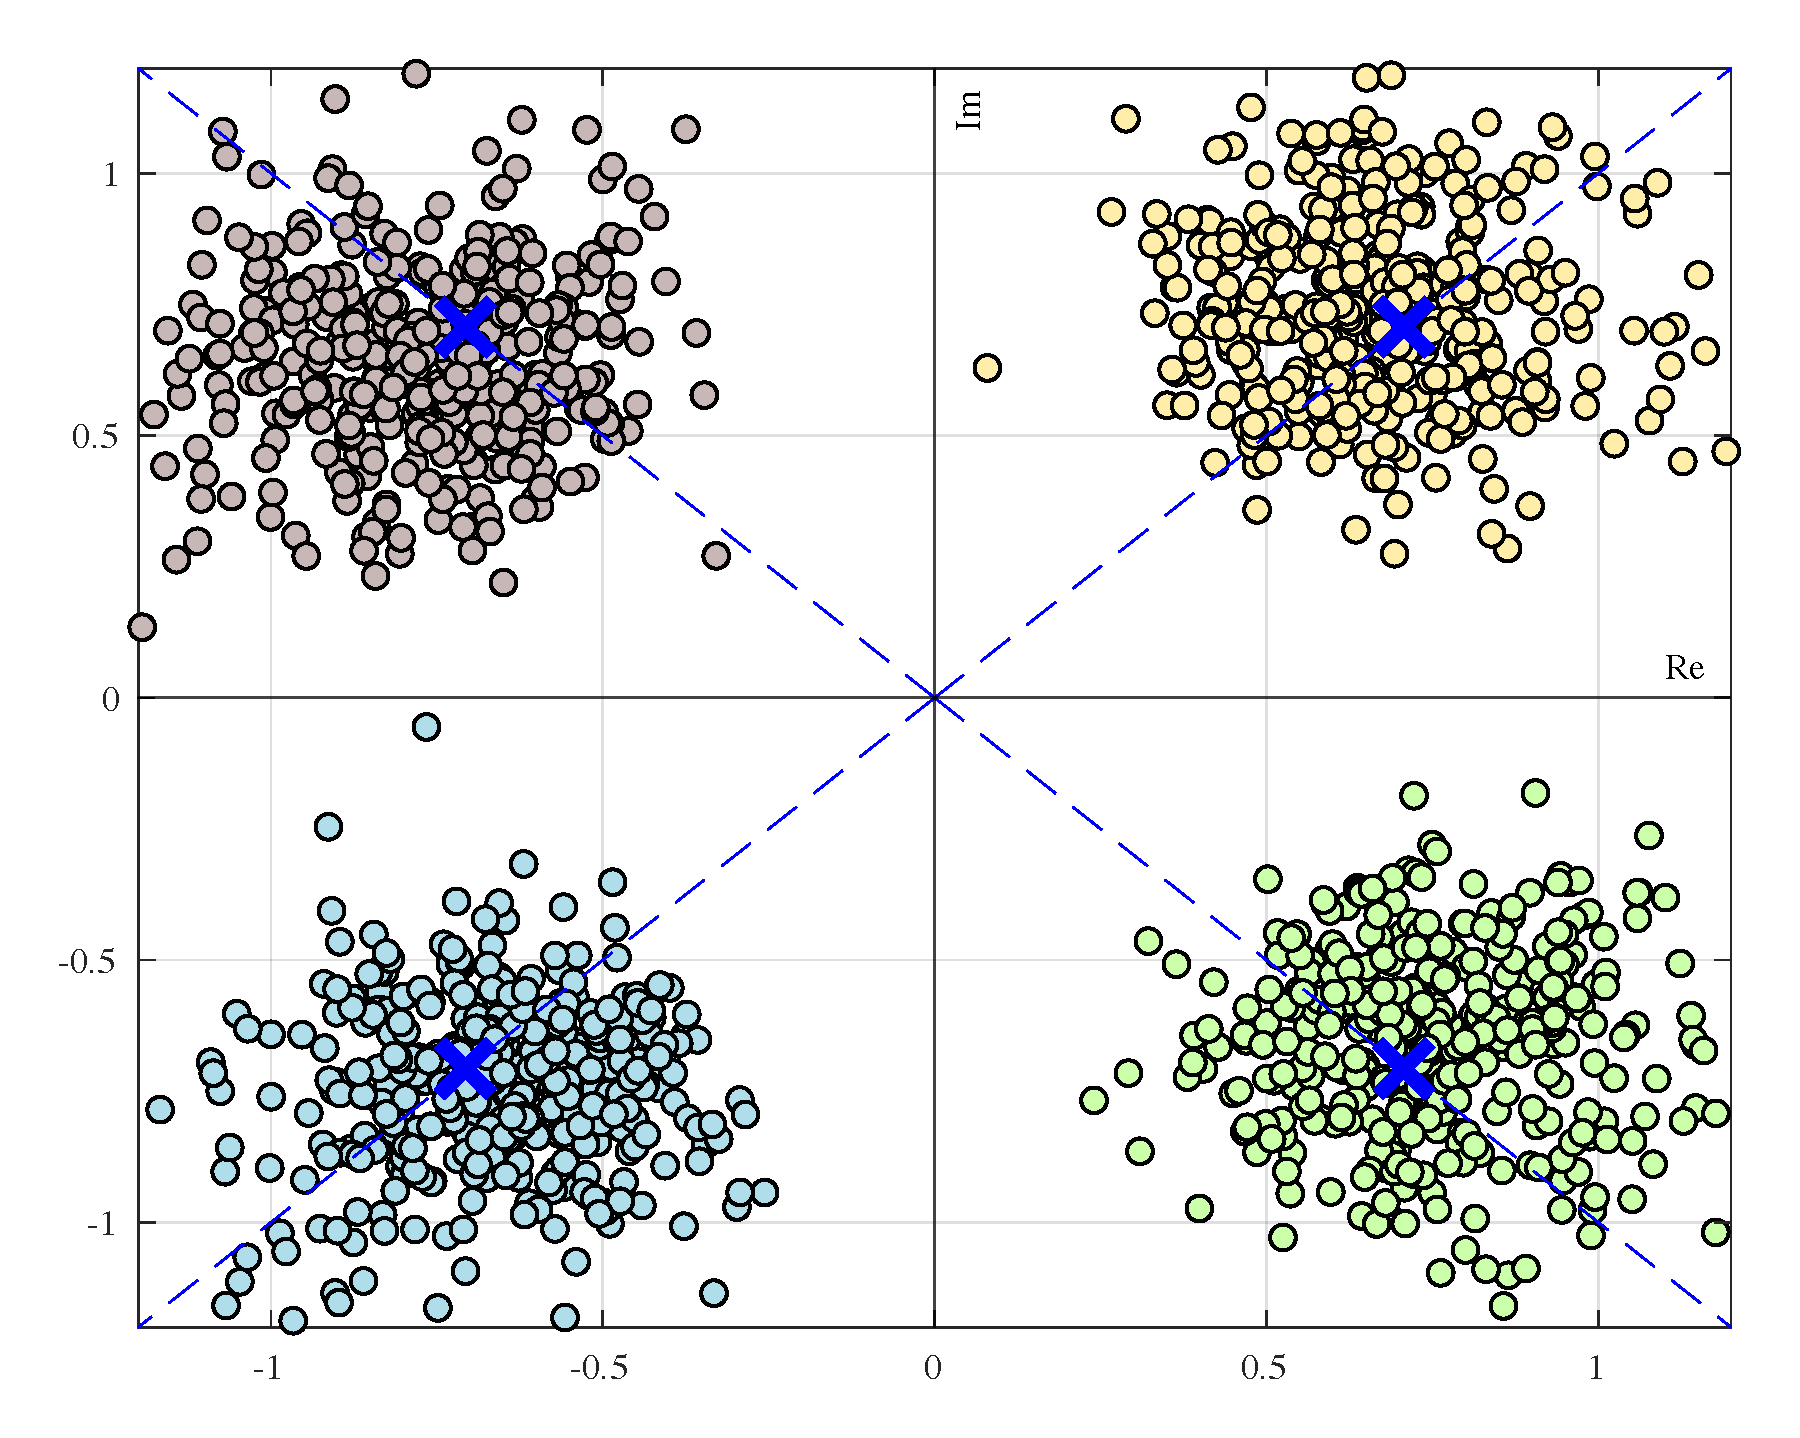
\includegraphics[width=0.8\linewidth]{dqpsk_snap-rtl.pdf}
  \caption{Graphic showing the assignment of \gls{dqpsk} data to one of four known values, based on the quadrant in which the data lies.}
  \label{fig:dqpsk_snap_rtl}
\end{figure}

The same data points are plotted against their corresponding carrier indices in Figure~\ref{fig:dqpsk_snap_rtl-alt}, with the snapped value lines and decision boundaries both shown. This is simply an alternative perspective of the previous plot.

\begin{figure}[htbp]
  \centering
  \captionsetup{type=figure}
  \def\svgwidth{\linewidth}
  {\setstretch{0.7} % Line spacing
      \input{../Images/dqpsk_snap_rtl-alt.pdf_tex}}
  \caption{Alternative plot of the \gls{dqpsk} snapping situation, viewed across the \(K\) carriers, showing the snapped values and decision boundaries.}
  \label{fig:dqpsk_snap_rtl-alt}
\end{figure}

In MATLAB, this snapping action was done by simply checking in which quadrant a point was, and assigning it to its correct value accordingly. For the function, this was performed for all points in the input matrix.

A graphical summary of the \texttt{dqpsk\_snap} function is shown in Figure~\ref{fig:dqpsk_snap}.

\begin{figure}[htbp]
  \centering
  \captionsetup{type=figure}
  \def\svgwidth{\linewidth}
  {\setstretch{0.7} % Line spacing
      \input{../Images/dqpsk_snap.pdf_tex}}
      \caption{Graphical summary of the \texttt{dqpsk\_snap} function.}
  \label{fig:dqpsk_snap}
\end{figure}

\subsection{Error Correction \label{subsect:dab-proc_error-correct}}
Though the snapping of the \gls{dqpsk} values was a straightforward way to eliminate the spreading in the phase data, it could not account for any errors that may have arisen in the signal. These errors could have come from various sources, including environmental noise and multipath effects. Moreover, some of the values in real-world data fell close to the decision boundary, and may have been assigned incorrectly. The \gls{dab} standard provides for this by integrating an error-correction method into any \gls{dab} signal, as described in the previous chapter during the discussion around \gls{fec}. Essentially, the transmitted data is convolutionally encoded, and can be decoded on the receiver's end with a Viterbi decoder.

Having said that, the original scope of this project did not include any error-correction implementation, and the sub-block is included here for completeness only. Ideally, in a fully-functional chain that is integrated into a \gls{pr} system, such functionality would indeed be included; however, its necessity depends on the quality of the \gls{dab} signals used in the system.

Conceptually, this sub-block would receive snapped \gls{dqpsk} data with the dimensions \((L-1)\times K\), and then output data with the same dimensions, after adjusting the possibly-erroneous values if necessary.

\section{Remodulation \label{sect:dab-proc_remodulate}}

\subsection{Overview}
The purpose of this block was to take the data output from the demodulation block, and modulate it anew, back into a \gls{dab} frame. Since the demodulated \gls{dqpsk} data was snapped, the output of the remodulation block was a perfectly reconstructed \gls{dab} signal\footnote{Owing to possible errors in the received signal, the reconstructed signal might not match the original, transmitted signal perfectly; instead, it is "perfectly reconstructed" in the sense of being a perfect \gls{dab} signal.}. Once again, this block was somewhat nugatory on its own, as it was specifically designed to be used in conjunction with the demodulator block.

Figure~\ref{fig:BD_Remod_All} shows a block diagram for the remodulation block, with the various sub-blocks, nomenclature, and dimensions shown.

\begin{figure}[htbp]
    \centering
    \captionsetup{type=figure}
    \def\svgwidth{\linewidth}
    {\setstretch{0.7} % Line spacing
        \input{../Images/BD_Remod_All-embed.pdf_tex}}
    \caption{Block diagram showing remodulation section of processing chain.}
    \label{fig:BD_Remod_All}
\end{figure}

The remodulation process had four key stages: firstly, the data points from the demodulation chain were interleaved in frequency, and then were mapped to a set of \gls{dab} carriers via \gls{dqpsk} modulation. Thereafter, the carriers were multiplexed into \gls{ofdm} symbols, and were finally packed into a single \gls{dab} frame.

Notice that these four sub-blocks in the remodulation chain were designed as inverses of the first four sub-blocks in the demodulation chain, shown previously in Figure~\ref{fig:BD_Demod_All}. For example, the first step in the demodulation block was \texttt{symbols\_unpack}, while the last step in the remodulation block was \texttt{symbols\_pack}, and so on. In fact, if perfect data was put through the chain---such that the \texttt{dqpsk\_snap} and \texttt{error\_correction} sub-blocks had no effect---the \texttt{demodulate} and \texttt{remodulate} functions would be perfectly symmetrical. This design choice was intentional, as it enabled a logical flow of operations, forwards and backwards through the chain, and also enabled individual blocks to be tested with their inverses---which will be discussed further in the validation chapter.

The details for each sub-block are given in the following sections.

\subsection{Frequency Interleaving \label{subsect:dab-proc_freq-interleave}}
The purpose of this sub-block was to re-interleave the data from the \texttt{demodulate} block, essentially to undo the effects of the \texttt{freq\_deinterleave} function. This process was termed frequency interleaving.
%Note that this sub-block could have been placed after the next sub-block, \texttt{dqpsk\_map}, without any changes in overall functionality, and if it was, the name would make more sense---as it would then be interleaving the \gls{dab} carriers, which are \emph{frequency} components. However, to create the conveninent forwards-backwards relationship for the demodulation and remodulation chains, its position was chosen as presented above. Thus, even though it was designed to interleave the \gls{dqpsk} data, its name was chosen to be consistent with the \gls{dab} standard's terminology~\cite{dabstandard}.

Interestingly, the same interleaving map as that created for the \texttt{freq\_deinterleave} functionality could be used here, only with a slightly different method of assigning the values. Whereas the previous function used the map to index elements on the right-hand side of the assignment, this function used the map to index elements on the left-hand side---see Listing~\ref{code:freq_interleave} for the code showing this. In this way, the same \texttt{build\_interleave\_map} tool could be used for both the interleaving and deinterleaving functionality. Note, however, that in the frequency interleaving function required knowledge the \gls{dab} mode, in order to pre-allocate the arrays correctly.

\begin{lstlisting}[caption={MATLAB code for the frequency interleaving functionality.},label={code:freq_interleave}]
function dab_data_interleaved = freq_interleave(dab_data, interleave_map, dab_mode)
  dab_data_interleaved = zeros(dab_mode.L-1,dab_mode.Tu);   % Pre-allocate space
  dab_data_interleaved(:,interleave_map) = dab_data;        % Use interleave map
end
\end{lstlisting}

In terms of dimensions, the sub-block received \((L-1)\) sets of \(K\) carriers, which it then transformed to \((L-1)\) sets of \(T_u\) carriers, with the middlemost and out-of-band carriers reintroduced with a value of 0. As was the case for frequency deinterleaving, visualizing the interleaving process was not particularly helpful---see Figure~\ref{fig:interleave_map} for a reminder of the messy interleaving map for Transmission Mode I. Nonetheless, the graphical summary of the functionality is given in Figure~\ref{fig:freq_deinterleave}.

\begin{figure}[htbp]
  \centering
  \captionsetup{type=figure}
  \def\svgwidth{\linewidth}
  {\setstretch{0.7} % Line spacing
  \input{../Images/freq_interleave.pdf_tex}}
  \caption{Graphical summary of the \texttt{frequency\_interleave} function.}
  \label{fig:freq_interleave}
\end{figure}

\subsection{DQPSK Mapping \label{subsect:dab-proc_dqpsk-map}}
With the \gls{dab} data values re-interleaved from the previous block, they were then used to modulate the \(T_u\) \gls{ofdm} carriers---a process termed \gls{dqpsk} mapping, in contrast to the demapping process discussed previously. Since differential modulation was used, the \((L-1)\) sets of \gls{dab} data at the input of the sub-block mapped to \(L\)~sets of \gls{dab} carriers. To provide a reference for the differential phase values, the \gls{prs} was assigned to be the first output symbol---recall that this was the other purpose of the \gls{prs}, in addition to the frame synchronization discussed previously. Consider Listing~\ref{code:dqpsk_map-1}, which shows the function set-up, with memory allocation and the assignment of the first symbol.

\begin{lstlisting}[caption={MATLAB code for setting up the \texttt{dqpsk\_map} function.},label={code:dqpsk_map-1}]
dab_carriers_remod = zeros(dab_mode.L, dab_mode.Tu); % Pre-allocate space
dab_carriers_remod(1,:) = prs; % First carrier is the phase reference symbol
\end{lstlisting}

With the first symbol then set, subsequent symbol values were calculated by mutliplying the previous symbol by the interleaved \gls{dab} data values for that index. Programmatically, this process was simple, and is shown in Listing~\ref{code:dqpsk_map-2}, where \texttt{dab\_data\_interleaved} was the output of the \texttt{freq\_interleave} sub-block.

\begin{lstlisting}[caption={MATLAB code for the actual \texttt{dqpsk\_map} functionality of differential modulation.},label={code:dqpsk_map-2}]
for l = 2:dab_mode.L
  dab_carriers_remod(l,:) = dab_data_interleaved(l-1,:) .* dab_carriers_remod(l-1,:);
end
\end{lstlisting}

Recall that the \gls{dab} data used in this sub-block ultimately came from the output of the demodulation block, which had snapped the \gls{dqpsk} values to one of four possible phase values, all with a magnitude of 1. As a consequence of this, the output of this \texttt{dqpsk\_map} sub-block was now "perfect," much like the data plotted in Figure~\ref{fig:ofdm-carriers-perfect}---that is, the resulting \gls{ofdm} symbols were now flat and rectangular in magnitude, and containing only four possible values in phase. Importantly, note that this was the case, even when using real-world data. Consider, for example, the illustration provided in Figure~\ref{fig:dqpsk_map-demo}, where the input \gls{ofdm} symbol was imperfect and had a high noise-floor; then, after being processed by the intervening blocks in the chain, the output \gls{ofdm} symbol was cleaned-up, with a low noise-floor and a perfectly rectangular magnitude.

\begin{figure}[htbp]
  \centering
  \captionsetup{type=figure}
  \def\svgwidth{\linewidth}
  {\setstretch{0.7} % Line spacing
    \input{../Images/dqpsk_map-demo.pdf_tex}}
  \caption{Demonstration of a section of the processing chain converting a noisy \gls{ofdm} symbol into a clean one.}
  \label{fig:dqpsk_map-demo}
\end{figure}

Graphically, the functionality of the \gls{dqpsk} mapping is shown in Figure~\ref{fig:dqpsk_map}. For clarity, the \texttt{phase\_reference\_symbol} input is coloured green, which corresponds to the first output of the \gls{dab} carriers.

\begin{figure}[htbp]
  \centering
  \captionsetup{type=figure}
  \def\svgwidth{\linewidth}
  {\setstretch{0.7} % Line spacing
  \input{../Images/dqpsk_map.pdf_tex}}
  \caption{Graphical summary of the \texttt{dqpsk\_map} function.}
  \label{fig:dqpsk_map}
\end{figure}

\subsection{OFDM Multiplexing \label{subsect:dab-proc_ofdm-mux}}
The purpose of this sub-block was to convert the modulated \gls{ofdm} carriers into time-domain signals, now reconstructed as perfect \gls{dab} signals. As explained in the \gls{ofdm} \emph{de}-multiplexing subsection, these two perspectives of the signal were, in fact, the same. However, since the data was being transformed from multiple signals from which data could easily be extracted (the \gls{ofdm} carriers), to single signals containing the sum of many carriers, this process was broadly termed "multiplexing."

As was the case for demultiplexing, the \gls{dft}/\gls{fft} could be used for easy extraction and reconstruction of the \gls{ofdm} symbols. Whereas the previous function used the a normal, forward \gls{fft}, this function used the \gls{ifft}---which is logical, considering the inverse relationship of the two blocks: one multiplexes, the other demultiplexes.

In code, this functionality looked mostly identical to that for the demultiplexing, shown previously in Listing~\ref{code:ofdm_demux}. Here, in Listing~\ref{code:ofdm_mux}, the only differences were that the \gls{ifft} was used, and the result was \emph{multiplied} by the length of the array, rather than being divided by it. Once again, this is logical, considering the inverse relationship.

\begin{lstlisting}[caption={MATLAB code for multiplexing an \gls{ofdm} symbol}, label={code:ofdm_mux}]
dab_symbols_remod = ifft(fftshift(dab_carriers_remod,2),[],2) .* length(dab_carriers_remod);
\end{lstlisting}

Since the \gls{ifft} is also a \(\mathbb{C}^N \to \mathbb{C}^N\) transformation, the \texttt{ofdm\_mux} function took an input of \(L\times T_u\) carriers, and output \(L\) symbols, each of length \(T_u\). A graphical summary of this functionality is provided in Figure~\ref{fig:ofdm_mux}.

\begin{figure}[htbp]
  \centering
  \captionsetup{type=figure}
  \def\svgwidth{\linewidth}
  {\setstretch{0.7} % Line spacing
  \input{../Images/ofdm_mux.pdf_tex}}
  \caption{Graphical summary of the \texttt{ofdm\_mux} function.}
  \label{fig:ofdm_mux}
\end{figure}

\subsection{Symbols Packing \label{subsect:dab-proc_symbols-pack}}
Finally, the purpose of this function was to take the matrix of remodulated \gls{dab} symbols, of size \(L \times T_u\), and transform it into a single array of the reconstructed \gls{dab} frame, with a total length of \(T_f\). In doing this, the sub-block was also responsible for adding the guard intervals and the null symbol.

Combining the guard interval for a particular symbol with the symbol itself was straightforward, as is shown in Listing~\ref{code:symbols_pack-1}, where \texttt{l} is the symbol index, and \texttt{dab\_symbols\_remod} is the data coming from the \texttt{ofdm\_mux} sub-block

\begin{lstlisting}[caption={},label={code:symbols_pack-1}]
lth_guard = dab_symbols_remod(l, end - dab_mode.Tg + 1 : end); % Last Tg values
lth_symbol = [lth_guard, dab_symbols_remod(l,:)]; % Full Symbol = [Guard , Original Symbol]
\end{lstlisting}

Packing the symbols then was a trivial process via a simple for-loop. Including the null symbol entailed simply padding the front of the array with \(T_\mathrm{null}\) zeros.

Graphically, this function is summarised in Figure~\ref{fig:symbols_pack}.

\begin{figure}[htbp]
  \centering
  \captionsetup{type=figure}
  \def\svgwidth{\linewidth}
  {\setstretch{0.7} % Line spacing
  \input{../Images/symbols_pack.pdf_tex}}
  \caption{Graphical summary of the \texttt{symbols\_pack} function.}
  \label{fig:symbols_pack}
\end{figure}

\section{Summary}
This chapter thoroughly explored the design of a \gls{dab} processing chain, starting with a high-level overview of the system via block diagrams, and later moving into the details of each block and sub-block. Plots were provided where appropriate, both to demonstrate the functionality of the code, and to provide a summarised graphical reference of each block, to be used when working with the chain. Short code snippets were given where necessary, in order to convey the essence of the chain's functioning. Longer form algorithms were provided for the frame synchronisation methods, since these were non-trivial.

% ----------------------------------------------------
\ifstandalone
\bibliography{../Bibliography/References.bib}
\printnoidxglossary[type=\acronymtype,nonumberlist]
\fi
\end{document}
% ----------------------------------------------------